\documentclass[12pt, a4paper]{article}
\usepackage[margin=1in]{geometry}
\usepackage{graphicx}
\usepackage{amsmath}
\usepackage{booktabs}
\usepackage{hyperref}
\usepackage{float}
\usepackage{multirow}
\usepackage[table]{xcolor}
\usepackage{setspace}
\usepackage{listings}
\usepackage{tikz}
\usetikzlibrary{shapes.geometric, arrows.meta, positioning, fit, backgrounds}
\graphicspath{{./}{results/plots/}}
\onehalfspacing

\lstset{
  basicstyle=\ttfamily\small,
  breaklines=true,
  frame=single,
  backgroundcolor=\color{gray!10},
  keywordstyle=\color{blue}\bfseries,
  commentstyle=\color{green!60!black},
  stringstyle=\color{red!70!black},
  numbers=left,
  numberstyle=\tiny\color{gray},
  showstringspaces=false
}

\title{\textbf{Smart Irrigation Scheduling Using Temporal-State-Aware\\Soft Actor-Critic Deep Reinforcement Learning}}
\author{
Joshika Somisetty, Padarthi Leela Sabareesh, Vobilisetti Vyvanth \\
Department of Artificial Intelligence \\
Amrita School of Artificial Intelligence, Bengaluru\\
Amrita Vishwa Vidyapeetham, India \\
\textit{Emails:}\\
\texttt{bl.en.u4aid23019@bl.students.amrita.edu}\\
\texttt{bl.en.u4aid23037@bl.students.amrita.edu}\\
\texttt{bl.en.u4aid23056@bl.students.amrita.edu}
}
\date{}

\begin{document}
\maketitle

\begin{abstract}
Agriculture consumes approximately 70\% of global freshwater, yet traditional irrigation strategies fail to adapt to dynamic environmental conditions. This paper presents a Temporal-State-Aware Soft Actor-Critic (TSA-SAC) deep reinforcement learning agent for optimizing irrigation scheduling in cotton cultivation. Our approach integrates a BiLSTM temporal encoder with attention mechanisms into the SAC framework. Evaluated in a custom physics-based environment (FAO-56 soil model + RUE crop growth), TSA-SAC achieves \$1,039/ha profit with only 1,152\,mm irrigation---outperforming the best expert heuristic by 5\% profit with 7\% less water. A six-variant ablation study confirms SAC outperforms PPO (+136\%) and DDPG (+2.5\%), while the TSA encoder contributes +1.7\% over MLP baselines.

\noindent\textbf{Keywords:} deep reinforcement learning, smart irrigation, soft actor-critic, BiLSTM, attention mechanism, water use efficiency
\end{abstract}

%================================================================
\section{Problem Statement}

Water scarcity constrains sustainable agricultural development globally. The agricultural sector accounts for approximately 70\% of freshwater withdrawals, with irrigation being the dominant use case. Against rising food demand driven by population growth, the challenge of producing more food with limited water has become a pressing issue.

Traditional irrigation strategies include: (1) \textit{fixed-schedule irrigation}, applying water at predetermined intervals regardless of crop needs, and (2) \textit{threshold-based methods}, triggering irrigation when soil moisture drops below a preset level. Both approaches are fundamentally reactive and suffer from several limitations:

\begin{itemize}
    \item They ignore dynamic weather patterns such as upcoming rainfall or temperature trends
    \item They do not account for varying water sensitivity across crop growth stages
    \item They cannot optimize for long-term seasonal water budget constraints
    \item They fail to capture complex interactions between soil, weather, and crop physiology
\end{itemize}

Cotton, our target crop, is particularly sensitive to water management. It has distinct growth stages (emergence, vegetative, flowering, boll formation, maturity) with varying water requirements. The flowering stage is critically water-sensitive---stress during this period causes irreversible yield loss. An intelligent system must learn to anticipate these needs and allocate water strategically across the entire 170-day growing season.

The core research question is: \textit{Can a deep reinforcement learning agent learn irrigation policies that achieve higher crop yields with less water than expert-designed heuristics?}

%================================================================
\section{Literature Survey}

\subsection{Traditional Irrigation Methods}
Fixed-schedule and threshold-based methods remain dominant in practice. Threshold methods using soil moisture sensors (e.g., irrigate when $\theta < 0.45$) perform better than fixed schedules but still apply a static rule regardless of weather forecasts, crop stage, or remaining water budget. Recent works have explored sensor fusion and IoT-based monitoring to improve threshold methods, though they remain inherently reactive \cite{zhang2021iot}.

\subsection{Machine Learning for Precision Agriculture}
Recent advances in machine learning have demonstrated strong potential for precision agriculture. Convolutional Neural Networks (CNNs) and Recurrent Neural Networks (RNNs) have been applied to crop yield prediction \cite{nevavuori2020crop} and disease detection. However, supervised learning methods require labeled historical data and cannot directly optimize long-term management strategies.

\subsection{Reinforcement Learning in Agriculture}
Chen et al.\ applied Q-learning to irrigation with discrete action spaces, demonstrating the feasibility of RL for agricultural control but limited by state discretization and tabular methods \cite{chen2021rl}. Deep Q-Networks later showed how neural value approximation can scale RL to high-dimensional state spaces \cite{mnih2015dqn}. Overweg et al.\ explored model-based RL with learned crop simulators, reducing dependence on expensive external simulators \cite{overweg2021crop}. Tao et al.\ proposed multi-objective RL frameworks that balance yield, water savings, and economic return \cite{tao2022multi}.

\subsection{Policy Gradient Methods}
Schulman et al.\ proposed Proximal Policy Optimization (PPO), an on-policy method applied to various control tasks \cite{schulman2017ppo}. However, PPO's sample inefficiency makes it challenging for long-horizon agricultural tasks where each episode spans an entire growing season. Fujimoto et al.\ introduced TD3 (Twin Delayed Deep Deterministic Policy Gradient) to address overestimation bias in actor-critic methods \cite{fujimoto2018td3}. Haarnoja et al.\ proposed Soft Actor-Critic (SAC), which maximizes both expected reward and policy entropy, providing better exploration and training stability \cite{haarnoja2018sac}.

\subsection{Temporal Sequence Modeling}
BiLSTM architectures have been successfully applied to sequential agricultural time series \cite{xu2020bilstm}. Attention mechanisms, particularly self-attention from the Transformer architecture \cite{vaswani2017}, have improved temporal feature extraction in crop growth modeling by weighting critical time steps more strongly.

\subsection{Deep RL for Resource Management}
Deep RL has been successfully applied to similar resource allocation tasks in smart grids \cite{xu2020energyrl} and water distribution networks \cite{mahler2020water}. These applications share the challenge of long-horizon sequential decision-making under uncertainty, similar to irrigation scheduling.

\subsection{Base Reference Paper}
Liu et al.\ (2025) proposed an intelligent irrigation scheduling method using the DSSAT crop model with an improved SAC agent featuring BiLSTM temporal encoding and attention mechanisms \cite{liu2025}. Their TSA-SAC architecture achieved 39\% improvement in water use efficiency over fixed-schedule strategies, demonstrating the value of temporal state representation in agricultural RL.

%================================================================
\section{Gaps and Challenges}

Despite recent progress, several key gaps remain in applying deep RL to irrigation scheduling:

\begin{enumerate}
    \item \textbf{Simulator dependency}: Most existing work relies on external crop simulators (DSSAT, AquaCrop) that are computationally expensive and not easily parallelizable for RL training, hindering large-scale experimentation.
    \item \textbf{Limited ablation studies}: Prior works lack systematic isolation of individual component contributions---BiLSTM encoding, attention weighting, and dynamic reward shaping---making it unclear which elements drive performance gains.
    \item \textbf{Poor generalization testing}: Few papers evaluate trained agents on unseen climate zones or water constraint levels, leaving generalization capability largely unknown.
    \item \textbf{Lack of algorithm comparison}: No systematic comparison of SAC vs.\ PPO vs.\ DDPG exists specifically in the irrigation domain, preventing informed algorithm selection.
    \item \textbf{Absent hyperparameter analysis}: Agricultural RL agents lack systematic sensitivity analyses, making it unclear which hyperparameters (learning rate, sequence length, hidden size) most impact performance.
    \item \textbf{Reward engineering complexity}: Designing reward functions that balance immediate yield with long-term water conservation across dynamic crop growth stages remains a challenge, with dynamic reward shaping adding instability risk.
\end{enumerate}

This work directly addresses gaps 1--5 by implementing a custom physics-based environment, conducting a six-variant ablation study, evaluating on four unseen conditions, providing systematic algorithm comparisons, and presenting hyperparameter sensitivity analysis.

%================================================================
\section{DRL Formulation}

We formulate irrigation scheduling as a Markov Decision Process (MDP) $(\mathcal{S}, \mathcal{A}, \mathcal{P}, \mathcal{R}, \gamma)$:

\subsection{State Space $\mathcal{S}$ (16-dimensional)}
The 16-dimensional observation vector is described in Table~\ref{tab:obs}.

\begin{table}[H]
\centering
\caption{Observation Space Components}
\label{tab:obs}
\begin{tabular}{clc}
\toprule
\textbf{Index} & \textbf{Variable} & \textbf{Range} \\
\midrule
0 & Leaf Area Index (normalized) & [0, 1] \\
1 & Biomass / max yield & [0, 1] \\
2 & Root depth / max depth & [0, 1] \\
3 & Available soil water & [0, 1] \\
4 & Reservoir level & [0, 1] \\
5 & Water stress factor ($1 - K_s$) & [0, 1] \\
6 & Reference ET ($\text{ET}_0$) & [0, 1] \\
7 & Today's rainfall & [0, 1] \\
8 & 3-day rainfall forecast & [0, 1] \\
9 & 3-day $\text{ET}_0$ forecast & [0, 1] \\
10--14 & Growth stage (one-hot encoding) & \{0, 1\} \\
15 & Seasonal budget remaining & [0, 1] \\
\bottomrule
\end{tabular}
\end{table}

Table~\ref{tab:obs} combines crop growth variables, soil-water status, weather information, crop stage indicators, and the remaining seasonal budget into a single normalized state representation. Including both current rainfall/ET and short-horizon forecasts allows the agent to anticipate upcoming water availability rather than reacting only to present soil moisture.

\subsection{Action Space $\mathcal{A}$}
Continuous irrigation depth: $a \in [0, 60]$ mm/day, implemented via tanh squashing:
\begin{equation}
    a = 30 \cdot \tanh(z) + 30
\end{equation}

\subsection{Reward Function $\mathcal{R}$}
The daily reward combines three objectives with stage-dependent weights:
\begin{equation}
    r_t = w_y \cdot \Delta_{\text{yield}} - w_w \cdot c_{\text{water}} \cdot s_{\text{scarcity}} - w_s \cdot (1 - K_s)^2
\end{equation}

Terminal reward at harvest ($t = T$):
\begin{equation}
    r_T = \frac{\text{yield} \times \text{price} - \text{irrigation} \times \text{cost} + \text{IWUE\_bonus}}{\text{scale}}
\end{equation}

The dynamic reward weights vary by growth stage---flowering receives higher yield weight ($w_y = 1.2$) and stress penalty ($w_s = 1.8$) to reflect its critical water sensitivity.

\subsection{SAC Objective}
SAC maximizes the entropy-regularized objective:
\begin{equation}
    J(\pi) = \sum_{t=0}^{T} \mathbb{E}\left[r_t + \alpha \mathcal{H}(\pi(\cdot|s_t))\right]
\end{equation}
where $\alpha$ is automatically tuned to maintain target entropy $\mathcal{H}_{\text{target}} = -\dim(\mathcal{A})$.

%================================================================
\section{RL Model}

\subsection{Soft Actor-Critic (SAC)}
SAC is an off-policy maximum entropy RL algorithm with the following components:
\begin{itemize}
    \item \textbf{Stochastic Actor} $\pi_\phi$: Outputs a squashed Gaussian distribution over actions
    \item \textbf{Twin Critics} $Q_{\theta_1}, Q_{\theta_2}$: Two independent Q-networks to reduce overestimation bias
    \item \textbf{Target Networks}: Soft-updated copies for stable Q-learning targets
    \item \textbf{Automatic Temperature} $\alpha$: Learned entropy coefficient balancing exploration and exploitation
\end{itemize}

The critic loss minimizes:
\begin{equation}
    L_Q = \mathbb{E}\left[\left(Q_\theta(s,a) - \left(r + \gamma \left(\min_{i=1,2} Q_{\bar\theta_i}(s', a') - \alpha \log \pi(a'|s')\right)\right)\right)^2\right]
\end{equation}

The actor loss maximizes:
\begin{equation}
    L_\pi = \mathbb{E}\left[\alpha \log \pi_\phi(a|s) - \min_{i=1,2} Q_{\theta_i}(s, a)\right]
\end{equation}

\subsection{TSA Encoder Architecture}

\subsubsection{BiLSTM Temporal Encoder}
A 2-layer Bidirectional LSTM processes the 7-day observation window $(B, 7, 16)$ into hidden representations $(B, 7, 2H)$:
\begin{equation}
    \vec{h}_t = \text{LSTM}_{\text{fwd}}(x_t, \vec{h}_{t-1}), \quad \overleftarrow{h}_t = \text{LSTM}_{\text{bwd}}(x_t, \overleftarrow{h}_{t+1})
\end{equation}
\begin{equation}
    h_t = [\vec{h}_t; \overleftarrow{h}_t] \in \mathbb{R}^{2H}
\end{equation}

\subsubsection{Temporal Attention}
Computes importance weights over the $T$ timesteps:
\begin{equation}
    \alpha_t = \text{softmax}\left(W_2 \cdot \tanh(W_1 \cdot h_t)\right), \quad c = \sum_{t=1}^{T} \alpha_t \cdot h_t
\end{equation}

\subsubsection{Feature Attention}
Operates over the feature dimension:
\begin{equation}
    \beta = \text{softmax}(W_4 \cdot \text{ReLU}(W_3 \cdot c)), \quad \hat{c} = c \odot \beta
\end{equation}

\subsection{Why SAC over PPO and DDPG?}
\begin{itemize}
    \item \textbf{vs.\ PPO}: SAC is off-policy (reuses past data via replay buffer), making it far more sample-efficient for long 170-day episodes
    \item \textbf{vs.\ DDPG}: SAC's entropy regularization prevents premature convergence and twin critics reduce overestimation
    \item \textbf{Continuous actions}: SAC naturally handles continuous irrigation amounts without discretization
\end{itemize}

%================================================================
\section{System Architecture}

\subsection{High-Level Architecture}
Figure~\ref{fig:arch} shows the overall system architecture. The system consists of three main components: a stochastic weather generator, a physics-based crop irrigation environment, and the TSA-SAC agent.

\begin{figure}[H]
\centering
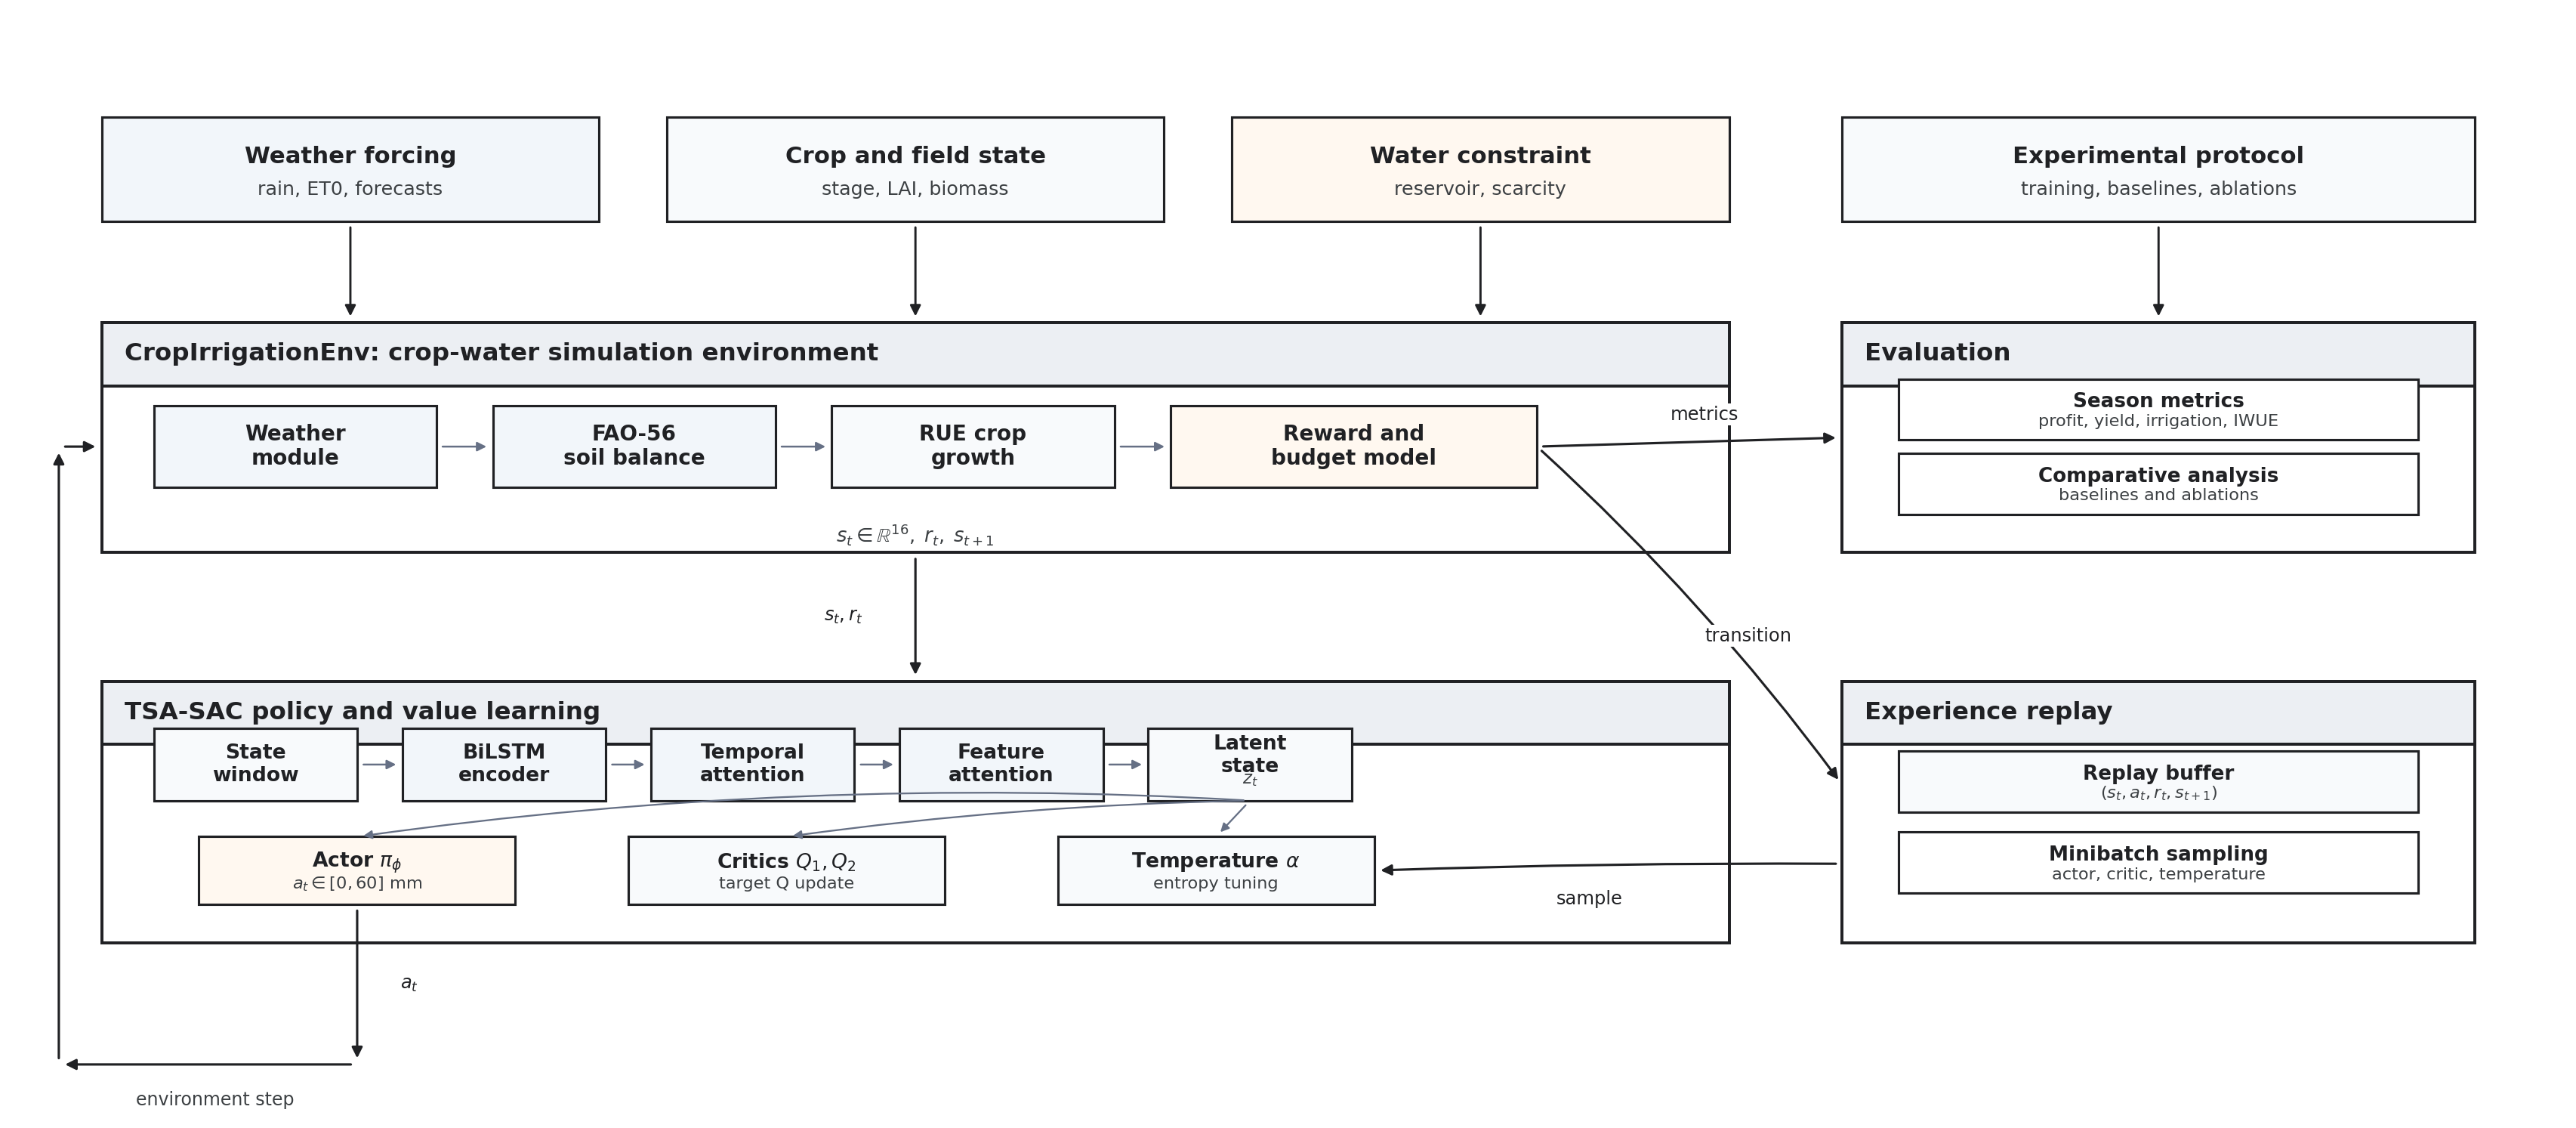
\includegraphics[width=0.95\textwidth]{system_architecture.png}
\caption{High-Level System Architecture of TSA-SAC Irrigation Scheduling}
\label{fig:arch}
\end{figure}

Figure~\ref{fig:arch} illustrates the closed-loop learning pipeline: exogenous weather, crop state, and water constraints drive the crop-water simulator; the simulator returns state and reward signals to the TSA-SAC agent; and the learned actor sends continuous irrigation actions back to the environment. The replay buffer supports off-policy updates, while the evaluation branch records season-level performance metrics.

\subsection{Detailed Agent Architecture}
The actor and critic networks each have their own independent BiLSTM encoder to prevent gradient interference. The attended context $\hat{c}$ feeds into a 2-layer MLP $(256, 256)$:
\begin{itemize}
    \item \textbf{Actor}: Outputs mean $\mu$ and log-std $\log\sigma$, producing actions via reparameterized sampling + tanh squashing
    \item \textbf{Twin Critics}: Each Q-network has its own independent BiLSTM encoder to prevent gradient interference
\end{itemize}


\subsection{Environment Architecture}
The custom Gymnasium-compatible environment (\texttt{environment.py}) implements:
\begin{itemize}
    \item A two-state Markov chain weather generator with sinusoidal temperature curves
    \item FAO-56 soil water balance with dynamic root depth and field capacity drainage
    \item A Radiation Use Efficiency (RUE) crop growth model with stage-sensitive LAI dynamics
    \item A seasonal water budget constraint with non-linear scarcity pricing
\end{itemize}

%================================================================
\section{Implementation Details}

\subsection{Custom Environment (\texttt{environment.py})}
We built a Gymnasium-compatible environment implementing:
\begin{itemize}
    \item \textbf{Weather Generator}: Two-state Markov chain for rainfall occurrence, gamma-distributed rainfall amounts, sinusoidal temperature curves with Gaussian noise
    \item \textbf{FAO-56 Soil Water Balance}: Dynamic root depth growth, field capacity drainage, effective rainfall/irrigation efficiency, water stress coefficient $K_s$ based on the FAO-56 evapotranspiration framework \cite{fao56}
    \item \textbf{RUE Crop Model}: Temperature and radiation-dependent biomass accumulation, stage-sensitive LAI dynamics
    \item \textbf{Water Budget}: Seasonal constraint with non-linear scarcity pricing---water becomes progressively more expensive as budget depletes
\end{itemize}

\subsection{Agent Implementation (\texttt{sac\_agent.py})}
Key implementation choices:
\begin{itemize}
    \item Sequence replay buffer storing $(s_{t-6:t}, a_t, r_t, s_{t-5:t+1}, d_t)$ tuples
    \item Huber loss for critic (more robust to outliers than MSE)
    \item Gradient clipping (max norm 1.0) for stability
    \item Automatic Mixed Precision (AMP) for GPU memory efficiency
    \item Alpha clamping in $[0.02, 0.5]$ to prevent entropy collapse
\end{itemize}

\subsection{Baseline Agents (\texttt{baselines.py})}
Four rule-based baselines were implemented for comparison:
\begin{itemize}
    \item \textbf{Random Policy}: Samples uniform random irrigation in $[0, 60]$ mm/day
    \item \textbf{Fixed Schedule (10-day)}: Applies 30\,mm every 10 days regardless of conditions
    \item \textbf{Threshold (0.45)}: Irrigates to field capacity when soil moisture drops below 45\%
    \item \textbf{Farmer Expert}: Stage-aware rule set applying known cotton heuristics
\end{itemize}

%================================================================
\section{Training}

\subsection{Training Configuration}
The hyperparameters used for training are listed in Table~\ref{tab:train}.

\begin{table}[H]
\centering
\caption{Training Hyperparameters}
\label{tab:train}
\begin{tabular}{ll}
\toprule
\textbf{Parameter} & \textbf{Value} \\
\midrule
Crop & Cotton (170-day season) \\
Climate & Arid (synthetic weather) \\
Training Episodes & 1000 \\
Reservoir Capacity & 2000\,mm \\
Water Budget & 1500\,mm (generous) \\
LSTM Hidden Size & 64 \\
LSTM Layers & 2 \\
MLP Hidden & (256, 256) \\
Learning Rate & $3 \times 10^{-4}$ \\
Sequence Length & 7 days \\
Replay Buffer Size & 1,000,000 \\
Batch Size & 64 \\
Discount ($\gamma$) & 0.99 \\
Soft Update ($\tau$) & 0.005 \\
\bottomrule
\end{tabular}
\end{table}

Table~\ref{tab:train} defines the main experimental setting used for the reported TSA-SAC results. The 7-day sequence length gives the temporal encoder enough context to observe recent rainfall and ET trends, while the large replay buffer supports stable off-policy learning across the long 170-day crop season.

\subsection{Training Convergence}
Key observations from training:
\begin{itemize}
    \item \textbf{Reward}: Converges from $\sim$0 to $\sim$250 by episode 150
    \item \textbf{Profit}: Rises from \$0 to $\sim$\$1,000 by episode 200
    \item \textbf{Irrigation}: Decreases from 1,500\,mm to $\sim$1,100\,mm as agent learns water conservation
    \item \textbf{Entropy $\alpha$}: Auto-tunes from 0.2 to $\sim$0.02, reducing exploration as policy stabilizes
    \item \textbf{Critic Loss}: Rises during exploration, then steadily decreases indicating value convergence
\end{itemize}

The training curves are shown in Figure~\ref{fig:training}. Figure~\ref{fig:agent} provides a detailed view of the critic loss, actor loss, and entropy coefficient over the course of training.

\begin{figure}[H]
\centering
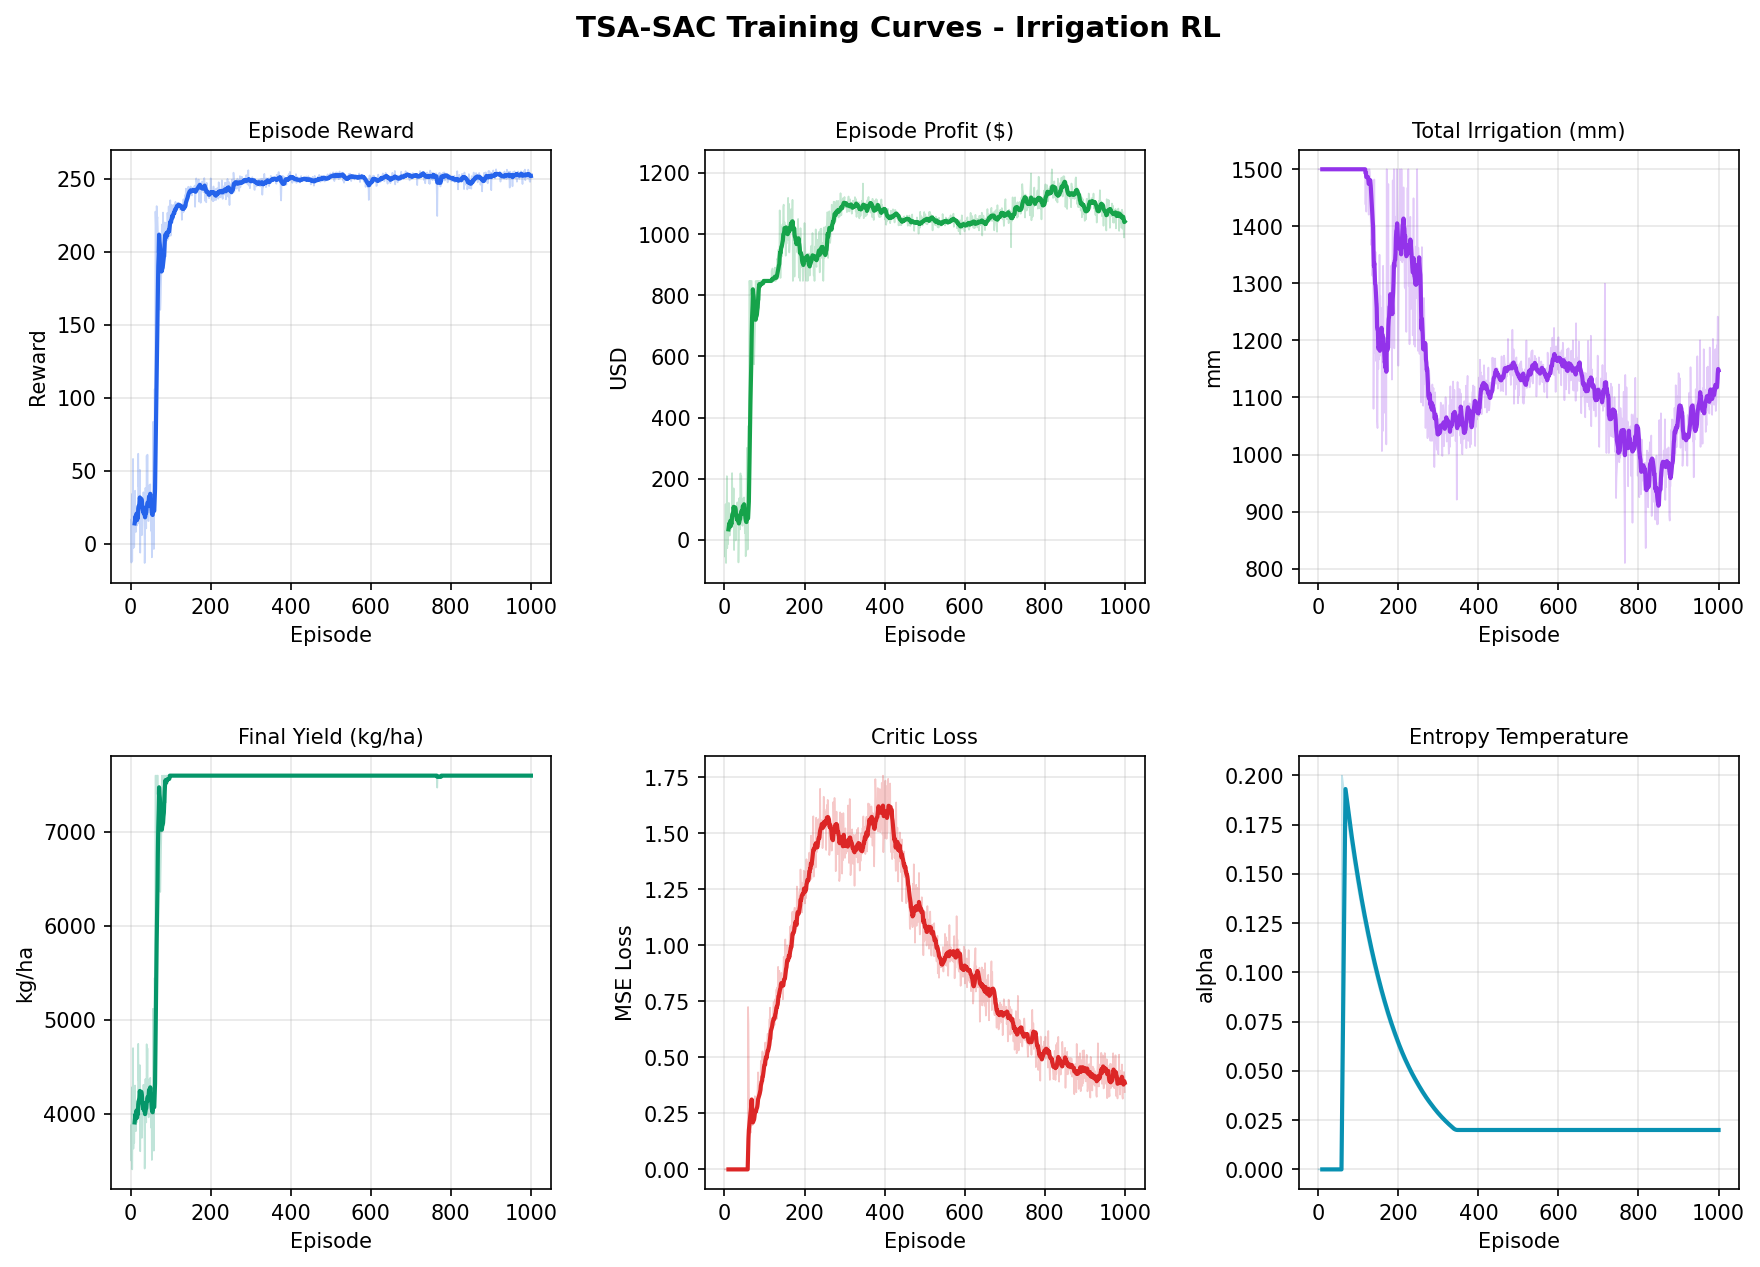
\includegraphics[width=0.95\textwidth]{training_curves.png}
\caption{TSA-SAC Training Curves over 1000 Episodes}
\label{fig:training}
\end{figure}

As seen in Figure~\ref{fig:training}, the agent transitions from random exploration to stable performance within approximately 200 episodes. Profit rises sharply from \$0 to \$1,000, while irrigation usage decreases from the maximum budget to $\sim$1,100\,mm, indicating that the agent learns to conserve water while maintaining yield.

\begin{figure}[H]
\centering
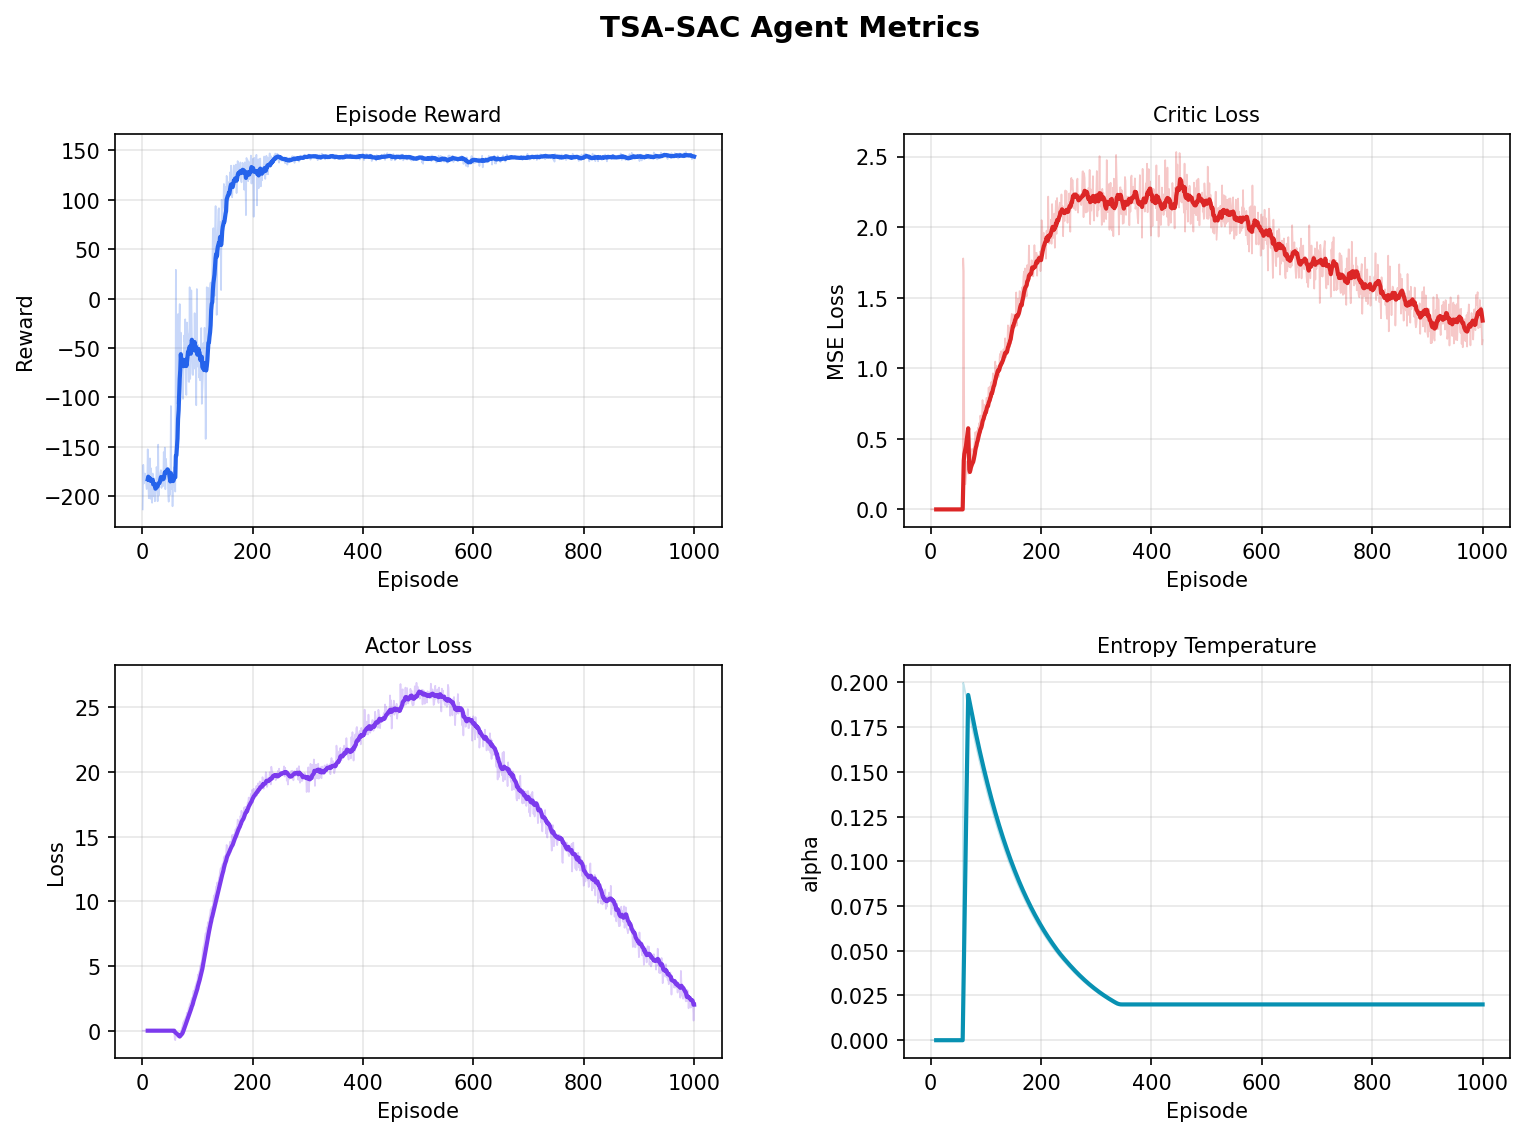
\includegraphics[width=0.85\textwidth]{agent_metrics.png}
\caption{Agent Metrics: Reward, Critic Loss, Actor Loss, and Entropy}
\label{fig:agent}
\end{figure}

Figure~\ref{fig:agent} reveals the internal training dynamics. The entropy coefficient $\alpha$ decays from 0.2 to $\sim$0.02 as the policy becomes more confident. Critic loss initially spikes during the exploration phase but steadily decreases as the value estimates stabilise, confirming healthy convergence.

%================================================================
\section{Hyperparameter Tuning}

Hyperparameter sensitivity was evaluated under a moderate water budget (400\,mm) using 100-episode training runs to stress-test the agent and reveal meaningful performance differences. The results are summarised in Table~\ref{tab:hp} and visualised in Figure~\ref{fig:hp}.

\begin{table}[H]
\centering
\caption{Hyperparameter Sensitivity Analysis}
\label{tab:hp}
\begin{tabular}{llc}
\toprule
\textbf{Parameter} & \textbf{Value} & \textbf{Profit (\$)} \\
\midrule
\multirow{3}{*}{Learning Rate} & $1 \times 10^{-4}$ & 720.6 \\
 & $3 \times 10^{-4}$ (default) & \textbf{763.3} \\
 & $1 \times 10^{-3}$ & 757.4 \\
\midrule
\multirow{3}{*}{LSTM Hidden} & 32 & 755.0 \\
 & 64 (default) & 754.6 \\
 & 128 & \textbf{775.4} \\
\midrule
\multirow{3}{*}{Sequence Length} & 1 (no history) & 632.7 \\
 & 3 days & 695.9 \\
 & 7 days (default) & \textbf{727.6} \\
\bottomrule
\end{tabular}
\end{table}

Table~\ref{tab:hp} shows that temporal context is the most influential tested factor: increasing the observation history from one day to seven days improves profit by roughly 15\%. Learning rate and LSTM hidden size also affect performance, but their differences are smaller, indicating that the agent is more sensitive to temporal information than to moderate capacity changes.

\begin{figure}[H]
\centering
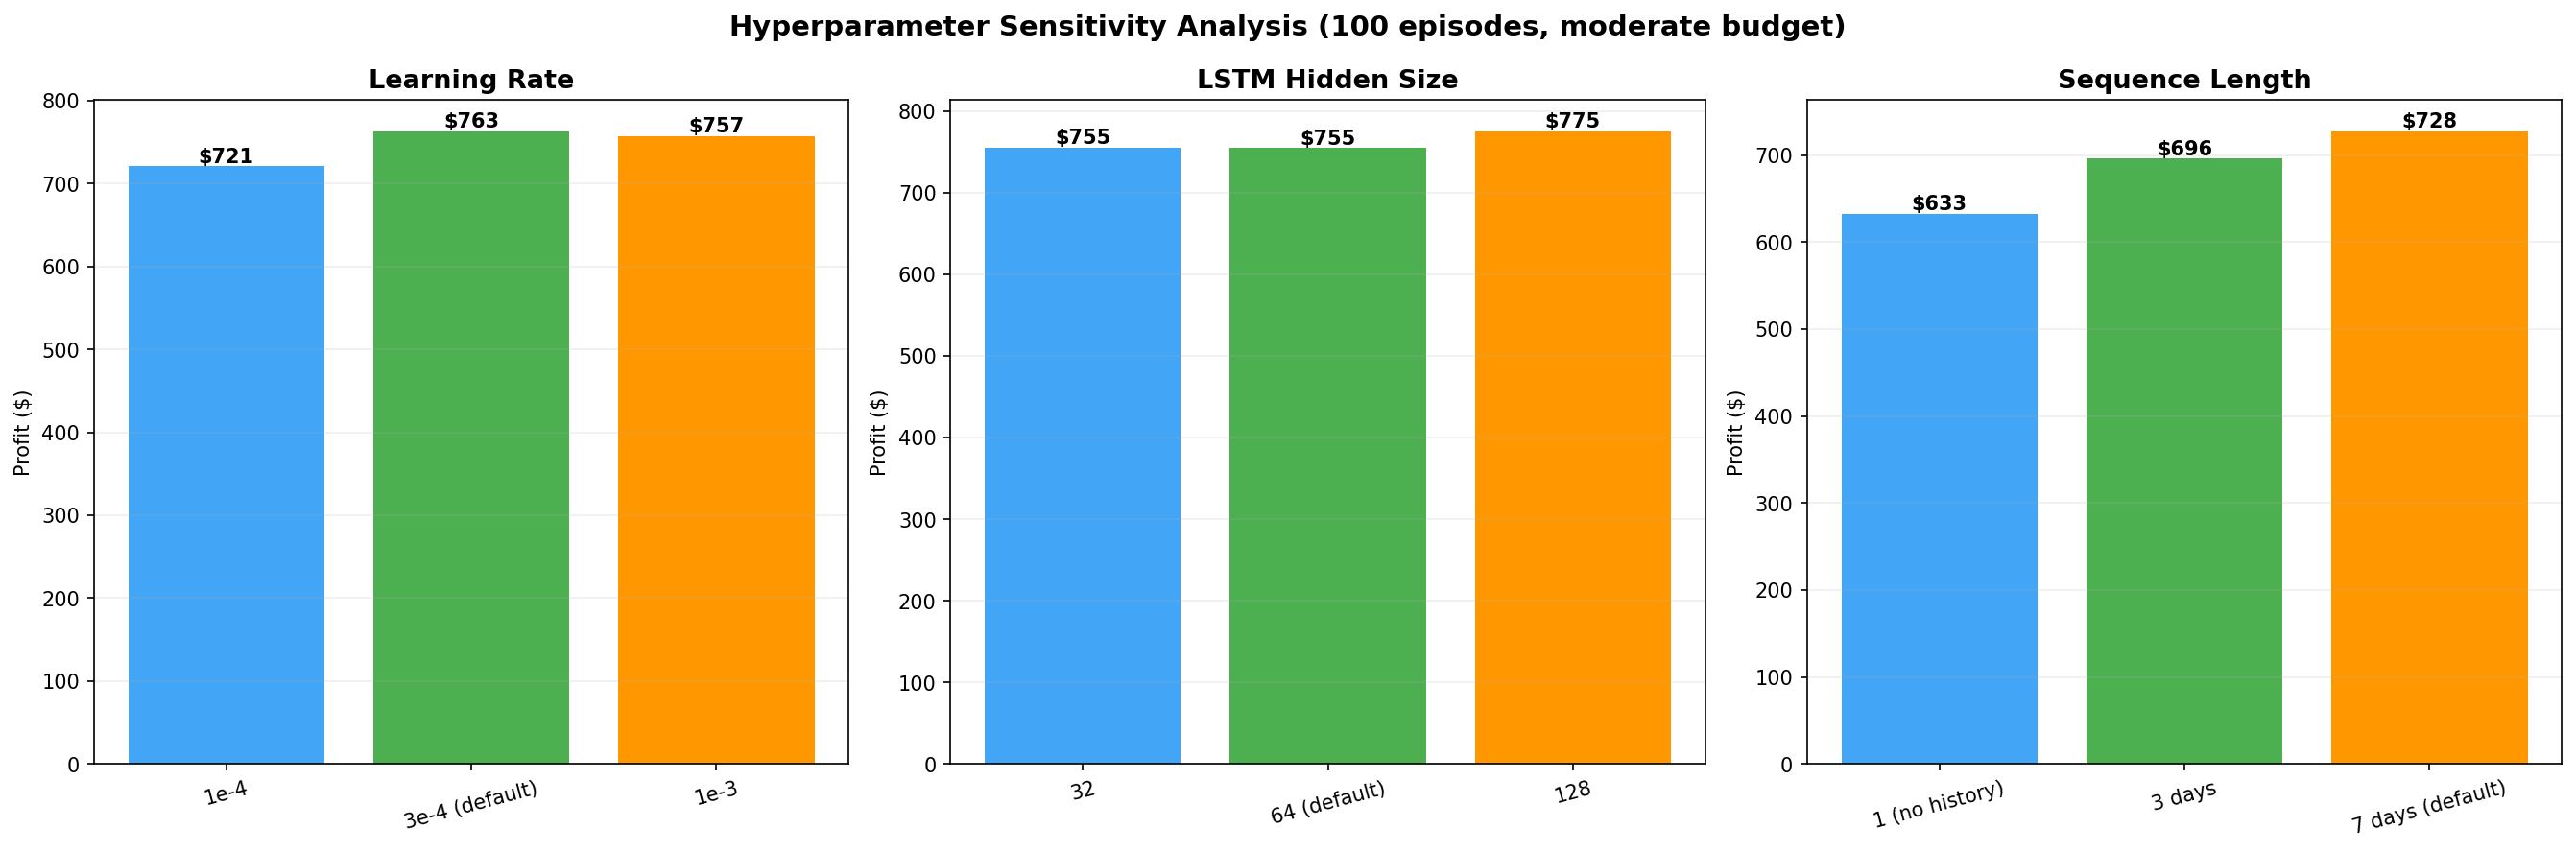
\includegraphics[width=0.95\textwidth]{hyperparameter_sensitivity.png}
\caption{Hyperparameter Sensitivity Analysis (100 episodes, 400\,mm budget)}
\label{fig:hp}
\end{figure}

Key observations:
\begin{itemize}
    \item \textbf{Learning Rate}: $3\times10^{-4}$ achieves the highest profit (\$763). Too low ($10^{-4}$) learns slowly; too high ($10^{-3}$) causes slight instability.
    \item \textbf{LSTM Hidden}: Larger hidden size (128) yields marginally better results (\$775 vs \$755), but at higher compute cost. The default 64 provides good efficiency.
    \item \textbf{Sequence Length}: 7-day history significantly outperforms no-history (\$728 vs \$633, +15\%), confirming the value of temporal context for weather-aware irrigation.
\end{itemize}

%================================================================
\section{Demo Code}

\subsection{Running the Demo Application}
The project ships with a Streamlit-based interactive dashboard (\texttt{demo\_app.py}) that allows live exploration of the trained TSA-SAC agent. To launch:

\begin{lstlisting}[language=bash, caption={Launching the Demo}]
# Install requirements
pip install -r requirements.txt

# Launch Streamlit dashboard
streamlit run demo_app.py
\end{lstlisting}

The demo includes five interactive tabs: (1) live simulation, (2) training curve visualization, (3) policy comparison, (4) ablation study results, and (5) architecture explanation.

\subsection{Training a New Agent}
\begin{lstlisting}[language=bash, caption={Training Commands}]
# Default training (cotton, arid, 1000 episodes)
python train.py

# Custom configuration
python train.py --crop cotton --climate arid --episodes 1000

# Evaluate a pre-trained checkpoint
python train.py --eval-only --model checkpoints/tsa_sac_improved_best.pt
\end{lstlisting}

\subsection{Key Code Snippet: TSA-SAC Agent}

The following snippet illustrates the core TSA-SAC action selection and training loop:

\begin{lstlisting}[language=Python, caption={TSA-SAC Core: Action Selection}]
class SACAgent:
    def select_action(self, seq, deterministic=False):
        """seq: np.ndarray of shape (seq_len, obs_dim)"""
        with torch.no_grad():
            seq_t = torch.FloatTensor(seq).unsqueeze(0)  # (1, T, obs_dim)
            mean, log_std = self.actor(seq_t)
            if deterministic:
                action = torch.tanh(mean) * 30 + 30
            else:
                std = log_std.exp()
                dist = torch.distributions.Normal(mean, std)
                z = dist.rsample()
                action = torch.tanh(z) * 30 + 30
        return action.squeeze().cpu().numpy()

    def update(self, batch):
        seqs, actions, rewards, next_seqs, dones = batch
        # ... twin critic + actor + alpha updates
        with autocast(device_type='cuda'):
            q1, q2 = self.critic(seqs, actions)
            target_q = rewards + self.gamma * (1 - dones) * \
                       (min_q_next - self.alpha * log_pi_next)
            critic_loss = F.huber_loss(q1, target_q) + \
                          F.huber_loss(q2, target_q)
        self.critic_optimizer.zero_grad()
        self.scaler.scale(critic_loss).backward()
        nn.utils.clip_grad_norm_(self.critic.parameters(), 1.0)
        self.scaler.step(self.critic_optimizer)
\end{lstlisting}

\subsection{Environment Reset and Step}
\begin{lstlisting}[language=Python, caption={Custom Environment Usage}]
from environment import CropIrrigationEnv

env = CropIrrigationEnv(
    crop="cotton",
    climate="arid",
    water_budget=1500,
    reservoir_capacity=2000,
    seed=42
)

obs, info = env.reset()
done = False
while not done:
    action = agent.select_action(obs_window)  # [0, 60] mm
    obs, reward, terminated, truncated, info = env.step(action)
    done = terminated or truncated

print(f"Season profit: ${info['profit']:.0f}/ha")
print(f"Total irrigation: {info['total_irrigation']:.0f} mm")
\end{lstlisting}

%================================================================
\section{Results and Discussion}

\subsection{Policy Comparison}
Table~\ref{tab:baseline} compares TSA-SAC against four baseline strategies. The results are visualised in Figure~\ref{fig:policy}, while the irrigation--yield tradeoff is shown in Figure~\ref{fig:tradeoff}.

\begin{table}[H]
\centering
\caption{Policy Comparison (Generous Budget, 30 Episodes)}
\label{tab:baseline}
\begin{tabular}{lccccc}
\toprule
\textbf{Policy} & \textbf{Profit (\$/ha)} & \textbf{Yield (kg/ha)} & \textbf{Irrig.\ (mm)} & \textbf{IWUE} & \textbf{Stress} \\
\midrule
Random & 237 & 4,825 & 1,500 & 3.22 & 93.2 \\
Farmer (10-day) & 836 & 5,713 & 765 & 7.47 & 81.0 \\
Threshold (0.45) & 946 & 7,600 & 1,320 & 5.76 & 0.0 \\
Farmer Expert & 990 & 7,600 & 1,240 & 6.13 & 0.0 \\
\textbf{TSA-SAC (ours)} & \textbf{1,039} & \textbf{7,600} & \textbf{1,152} & \textbf{6.60} & 16.0 \\
\bottomrule
\end{tabular}
\end{table}

TSA-SAC achieves the highest profit (\$1,039/ha) while using the least irrigation (1,152\,mm). Compared to Farmer Expert, TSA-SAC earns 5\% more profit with 7\% less water. The agent accepts 16 stress days (vs.\ 0 for heuristics) as a calculated trade-off---minor stress during non-critical stages saves water for critical periods.

\begin{figure}[H]
\centering
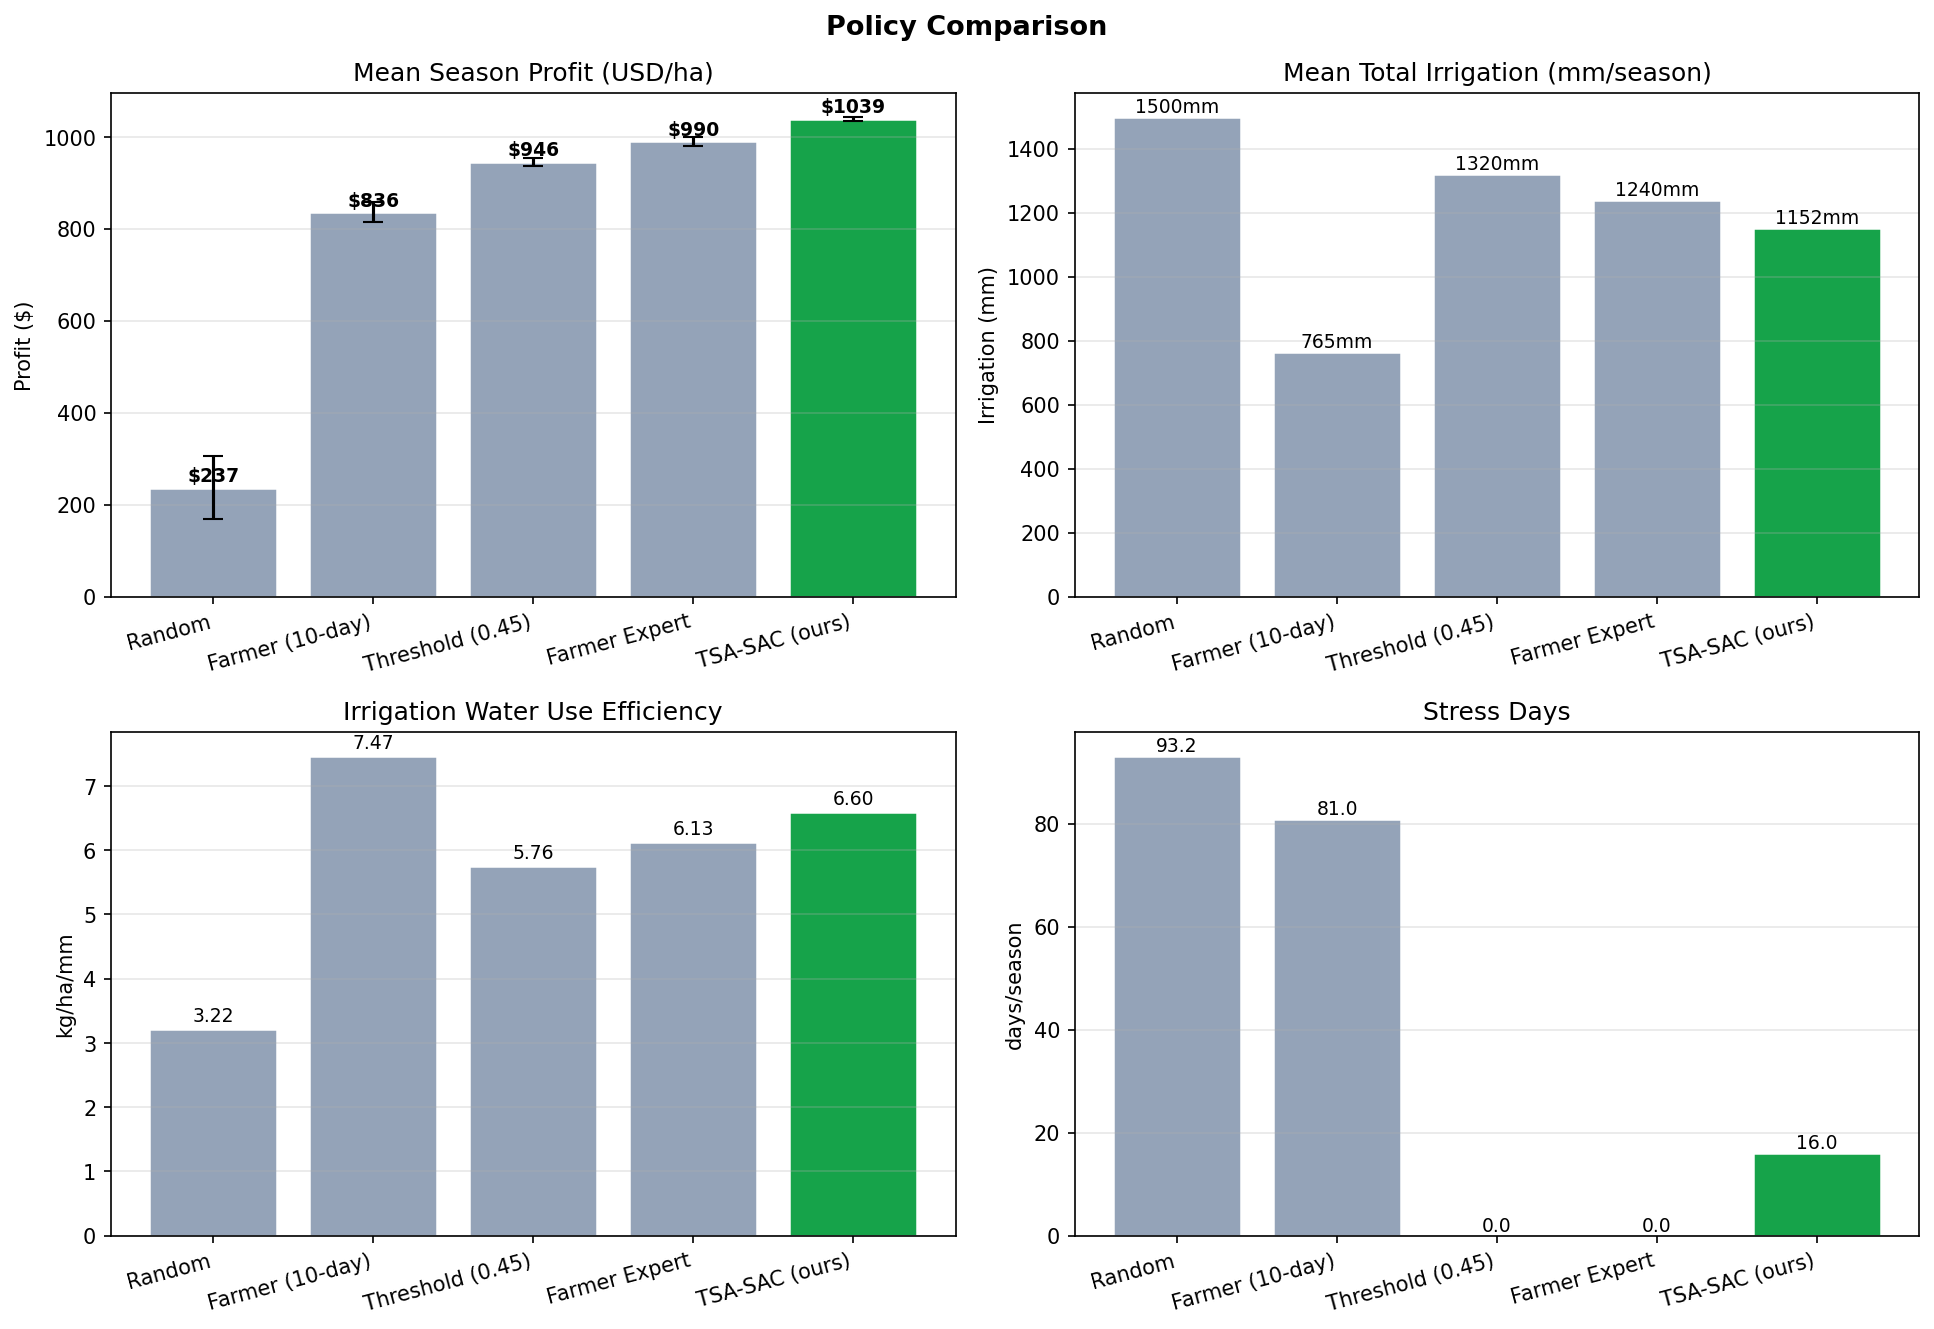
\includegraphics[width=0.95\textwidth]{policy_comparison.png}
\caption{Policy Comparison: Profit, Irrigation, IWUE, and Stress Days}
\label{fig:policy}
\end{figure}

Figure~\ref{fig:policy} shows that TSA-SAC dominates all four metrics. Notably, it achieves the highest IWUE (6.60\,kg/ha/mm) despite accepting a small number of stress days, illustrating the agent's learned ability to trade minor short-term stress for significant long-term water savings.

\begin{figure}[H]
\centering
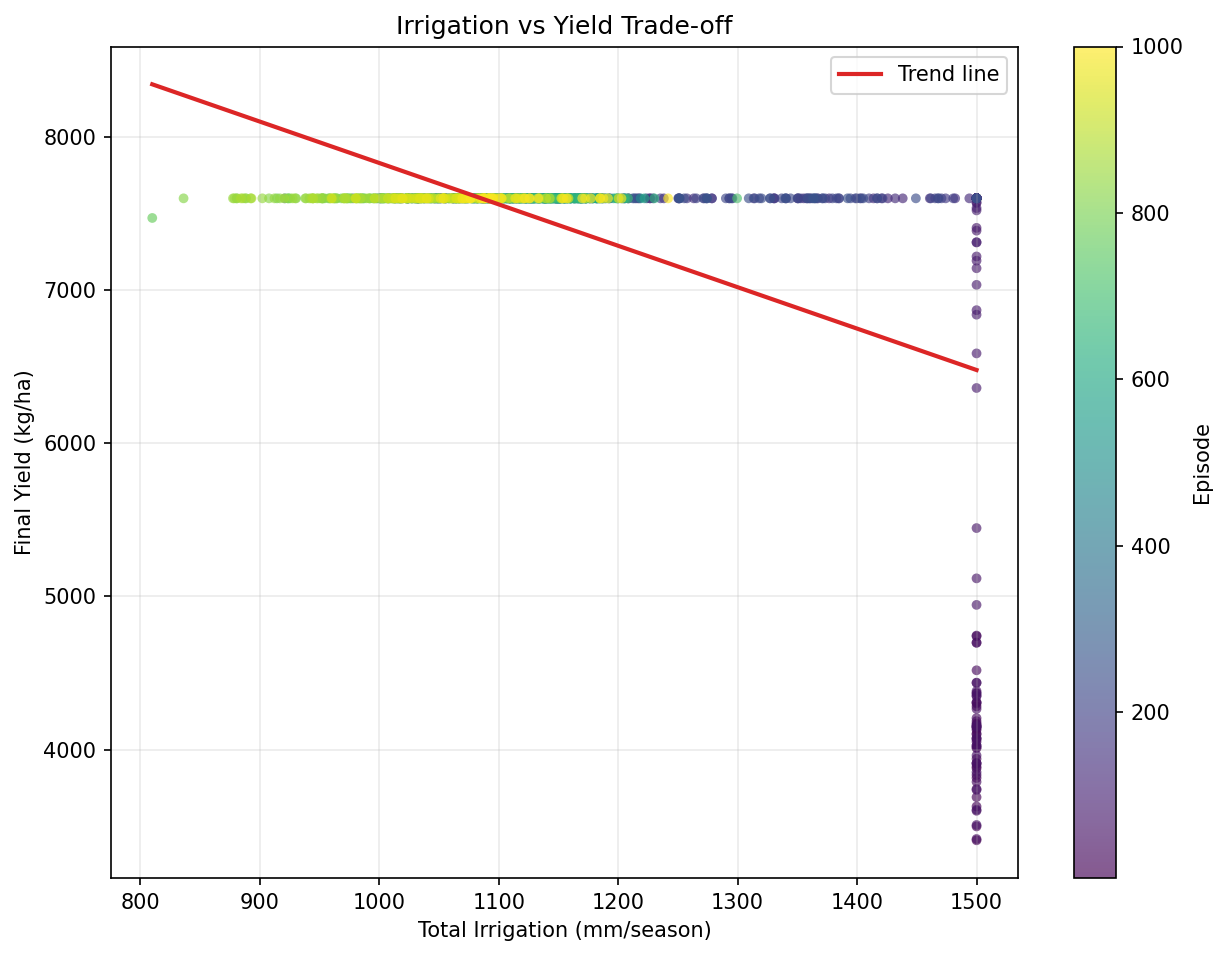
\includegraphics[width=0.8\textwidth]{irrigation_yield_tradeoff.png}
\caption{Irrigation--Yield Tradeoff across Policies}
\label{fig:tradeoff}
\end{figure}

Figure~\ref{fig:tradeoff} plots each policy in irrigation--yield space, revealing that TSA-SAC occupies the Pareto-optimal region: achieving maximum yield (7,600\,kg/ha) with the least irrigation. This confirms that the RL agent discovers more efficient scheduling than hand-crafted heuristics.

\subsection{Ablation Study}
To isolate the contribution of each architectural component, we conducted an ablation study with six variants trained for 500 episodes under a moderate water budget (400mm). The results are shown in Table~\ref{tab:ablation} with corresponding bar charts in Figure~\ref{fig:ablation} and learning curves in Figure~\ref{fig:ablation_lc}.

\begin{table}[H]
\centering
\caption{Ablation Study (400\,mm Budget, 500 Episodes, Seed=42)}
\label{tab:ablation}
\begin{tabular}{lcccc}
\toprule
\textbf{Variant} & \textbf{Profit (\$)} & \textbf{Yield (kg/ha)} & \textbf{IWUE} & \textbf{Stress Days} \\
\midrule
TSA-SAC (fixed reward) & \textbf{817} & \textbf{4,714} & 11.79 & 94.8 \\
SAC-MLP & 804 & 4,652 & 11.63 & 95.8 \\
SAC-BiLSTM & 803 & 4,651 & 11.63 & 95.8 \\
DDPG-MLP & 784 & 4,563 & 11.41 & 97.2 \\
TSA-SAC (dynamic) & 783 & 4,557 & 11.39 & 97.2 \\
PPO-MLP & 340 & 1,880 & 14.05 & 153.2 \\
\bottomrule
\end{tabular}
\end{table}

Key findings from the ablation:
\begin{itemize}
    \item \textbf{SAC $\gg$ PPO} (+136\%): SAC's off-policy learning and entropy regularization are critical for continuous irrigation control.
    \item \textbf{SAC $>$ DDPG} (+2.5\%): SAC's maximum entropy objective provides better exploration than DDPG's deterministic policy.
    \item \textbf{TSA encoder $>$ MLP} (+1.7\%): Temporal attention captures weather patterns that flat MLPs miss.
    \item \textbf{Fixed reward $>$ dynamic reward under constraint}: With limited water (400\,mm), the simpler fixed reward avoids risky exploration that dynamic stage-aware weights can induce.
\end{itemize}

Figure~\ref{fig:ablation} visualises the profit and yield comparison, clearly showing SAC-based variants clustered near the top while PPO lags significantly. Figure~\ref{fig:ablation_lc} displays the learning curves, confirming that SAC variants converge within 200 episodes whereas PPO fails to stabilise.

\begin{figure}[H]
\centering
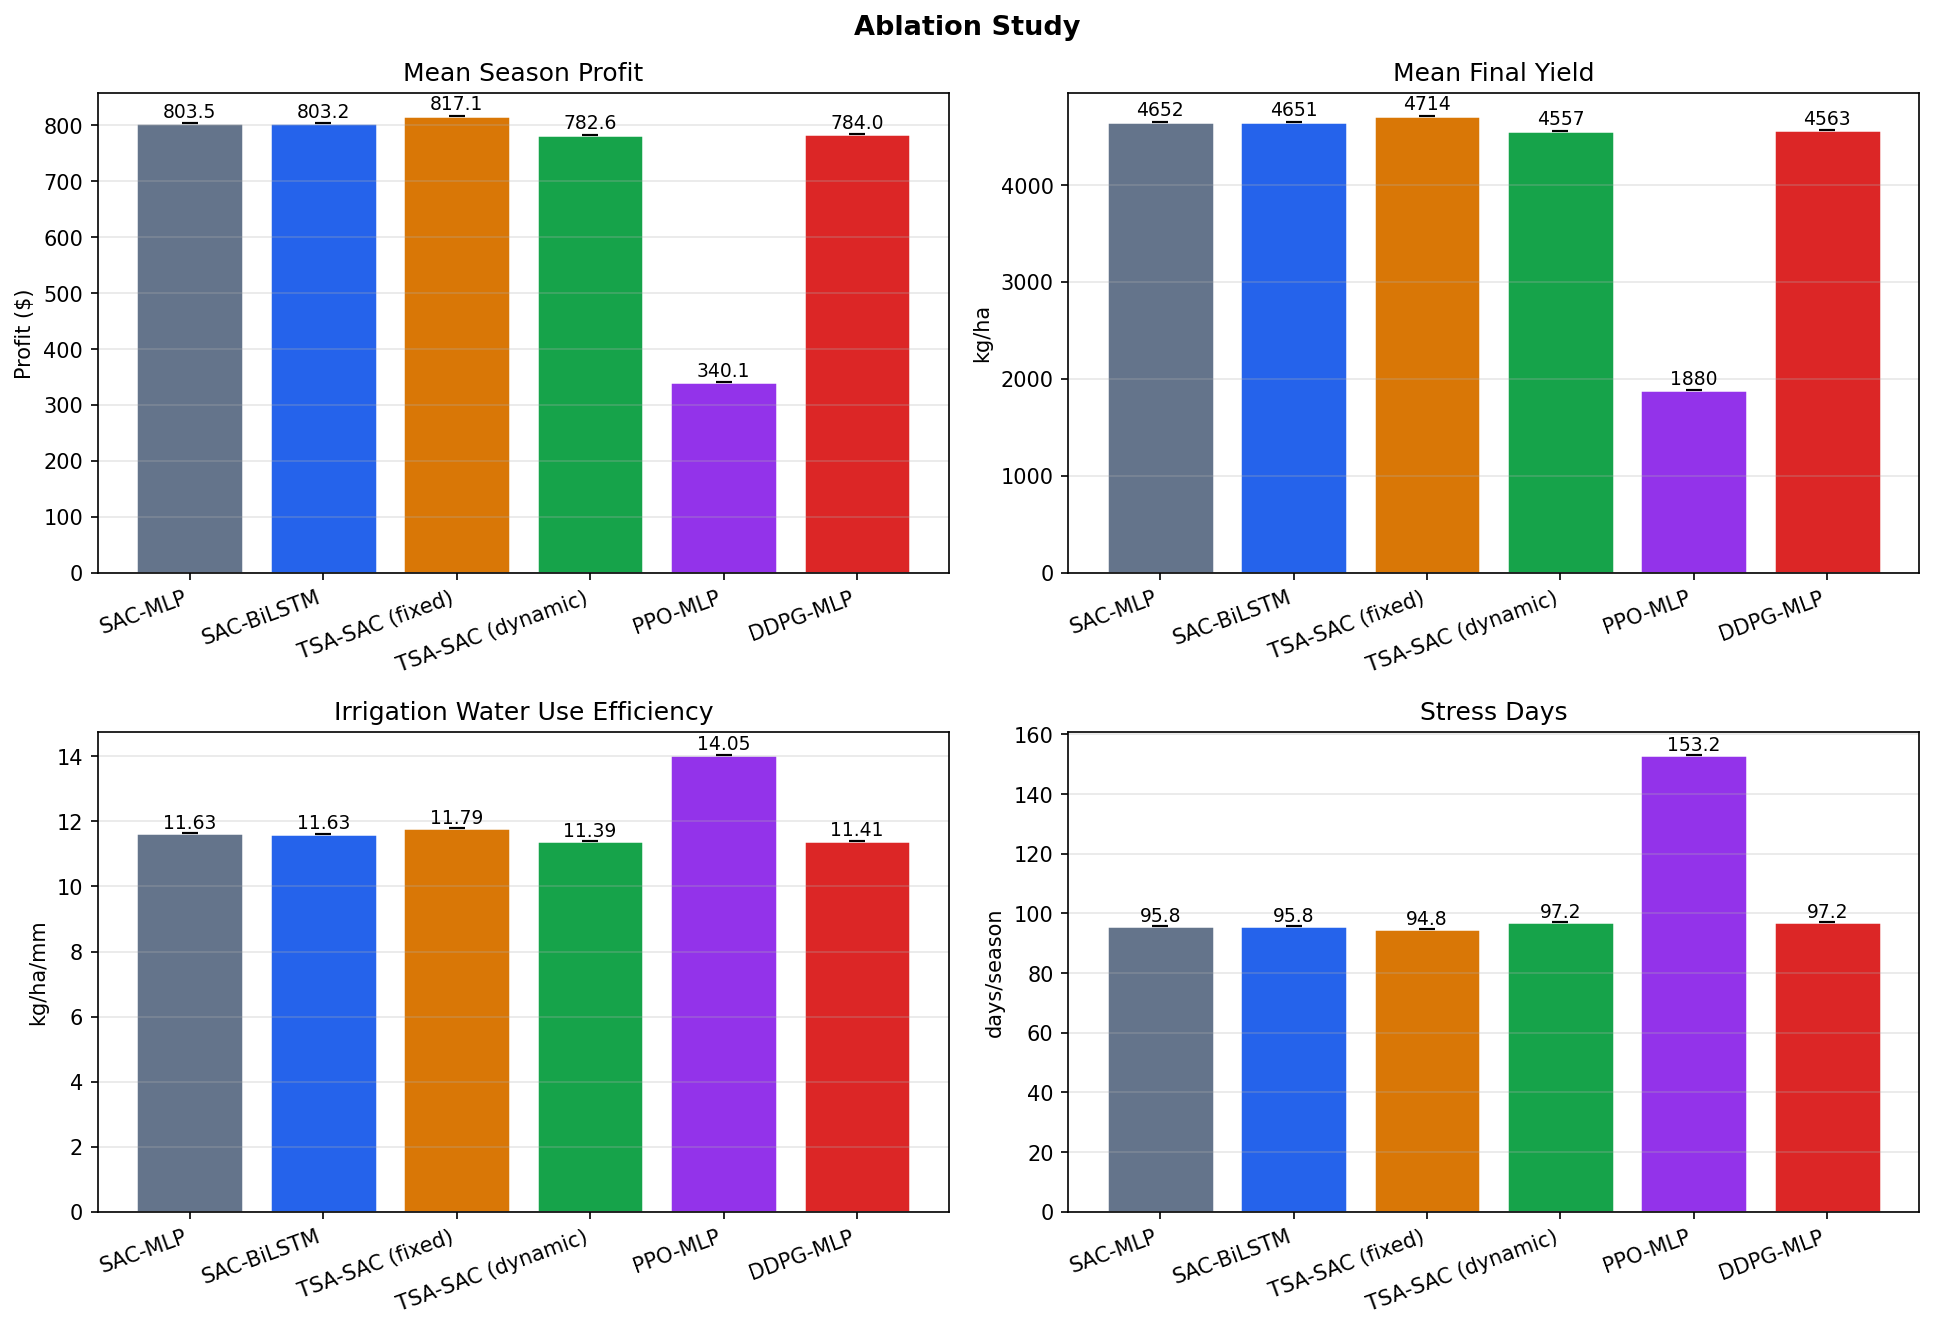
\includegraphics[width=0.95\textwidth]{ablation_study.png}
\caption{Ablation Study: Profit and Yield Comparison across Variants}
\label{fig:ablation}
\end{figure}

Figure~\ref{fig:ablation} summarizes the component-level contribution of each model variant. SAC-based methods consistently achieve higher profit and yield than PPO, while the fixed-reward TSA-SAC variant provides the strongest performance under the moderate water constraint.

\begin{figure}[H]
\centering
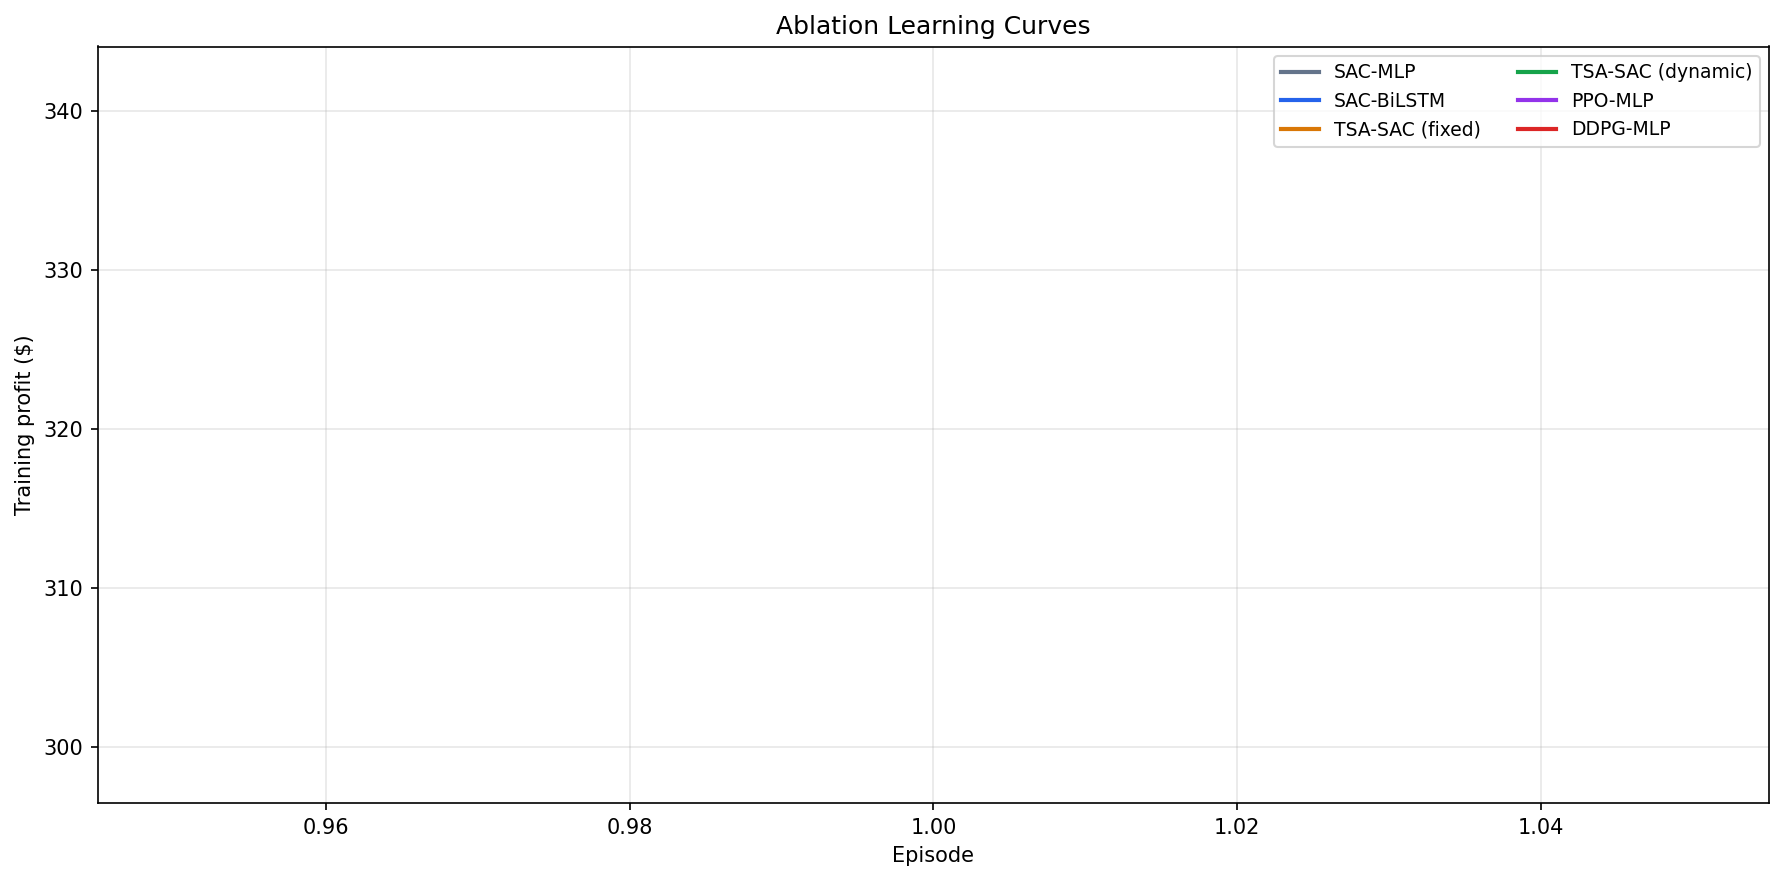
\includegraphics[width=0.95\textwidth]{ablation_learning_curves.png}
\caption{Ablation Learning Curves: Training Progression for Each Variant}
\label{fig:ablation_lc}
\end{figure}

The learning curves in Figure~\ref{fig:ablation_lc} show that all SAC-based variants converge within 200 episodes, while PPO-MLP remains flat with high variance even after 500 episodes. This confirms that off-policy learning is essential for the long-horizon irrigation scheduling task where each episode spans 170 days.

\subsection{Unseen Environment Generalization}
The trained agent (arid climate) was evaluated on four unseen environment configurations. Table~\ref{tab:unseen} presents the quantitative results, while Figure~\ref{fig:unseen} and Figure~\ref{fig:robust} visualise the performance degradation across environments.

\begin{table}[H]
\centering
\caption{Generalization to Unseen Environments}
\label{tab:unseen}
\begin{tabular}{lcccc}
\toprule
\textbf{Scenario} & \textbf{Profit (\$)} & \textbf{Yield (kg/ha)} & \textbf{IWUE} & \textbf{Stress Days} \\
\midrule
Trained (arid, generous) & \textbf{1,201} & 7,600 & 8.88 & 46.0 \\
Best: humid, generous & 1,000 & 5,875 & 11.05 & 0.0 \\
Avg: semi-arid, moderate & 860 & 4,908 & 12.27 & 77.5 \\
Worst: arid, scarce & 588 & 3,296 & 13.18 & 117.3 \\
\bottomrule
\end{tabular}
\end{table}

The agent generalizes well across unseen conditions. In humid climates, it achieves zero stress days by leveraging natural rainfall. Under scarce budgets, profit degrades gracefully (\$588 vs \$1,201) rather than catastrophically, demonstrating learned robustness.

\begin{figure}[H]
\centering
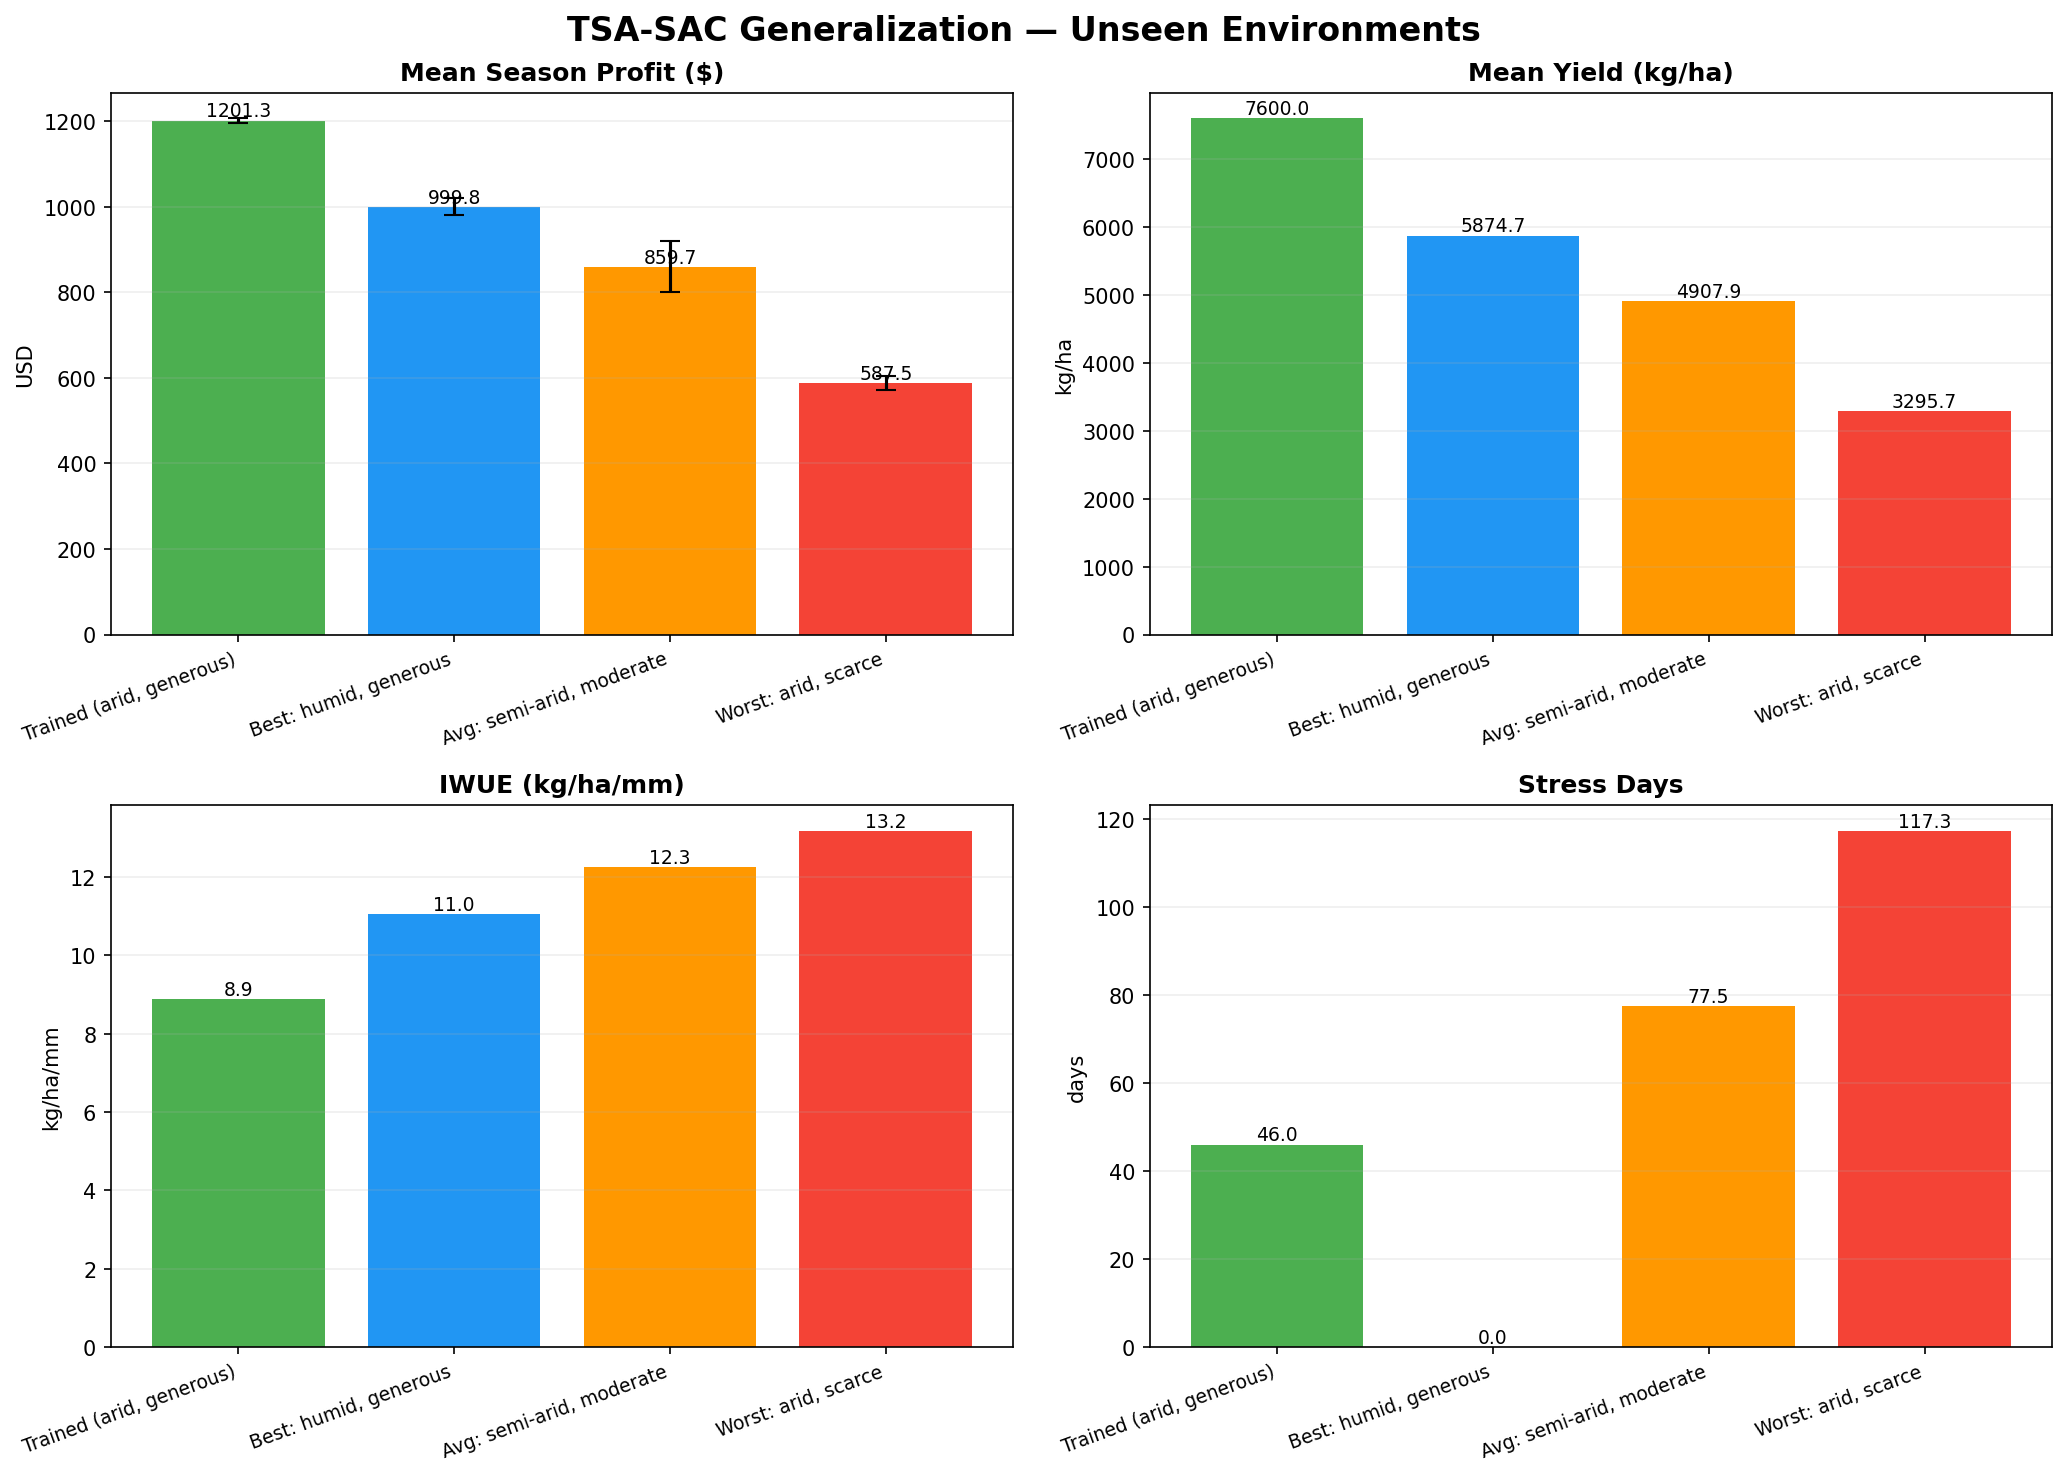
\includegraphics[width=0.95\textwidth]{unseen_environment.png}
\caption{Generalization Performance across Unseen Environments}
\label{fig:unseen}
\end{figure}

Figure~\ref{fig:unseen} shows that performance declines as climates become drier and water budgets become stricter, but the policy still preserves meaningful profit and yield in the most constrained scenario. This indicates that the learned strategy generalizes beyond the exact training condition instead of overfitting to a single arid, generous-budget environment.

\begin{figure}[H]
\centering
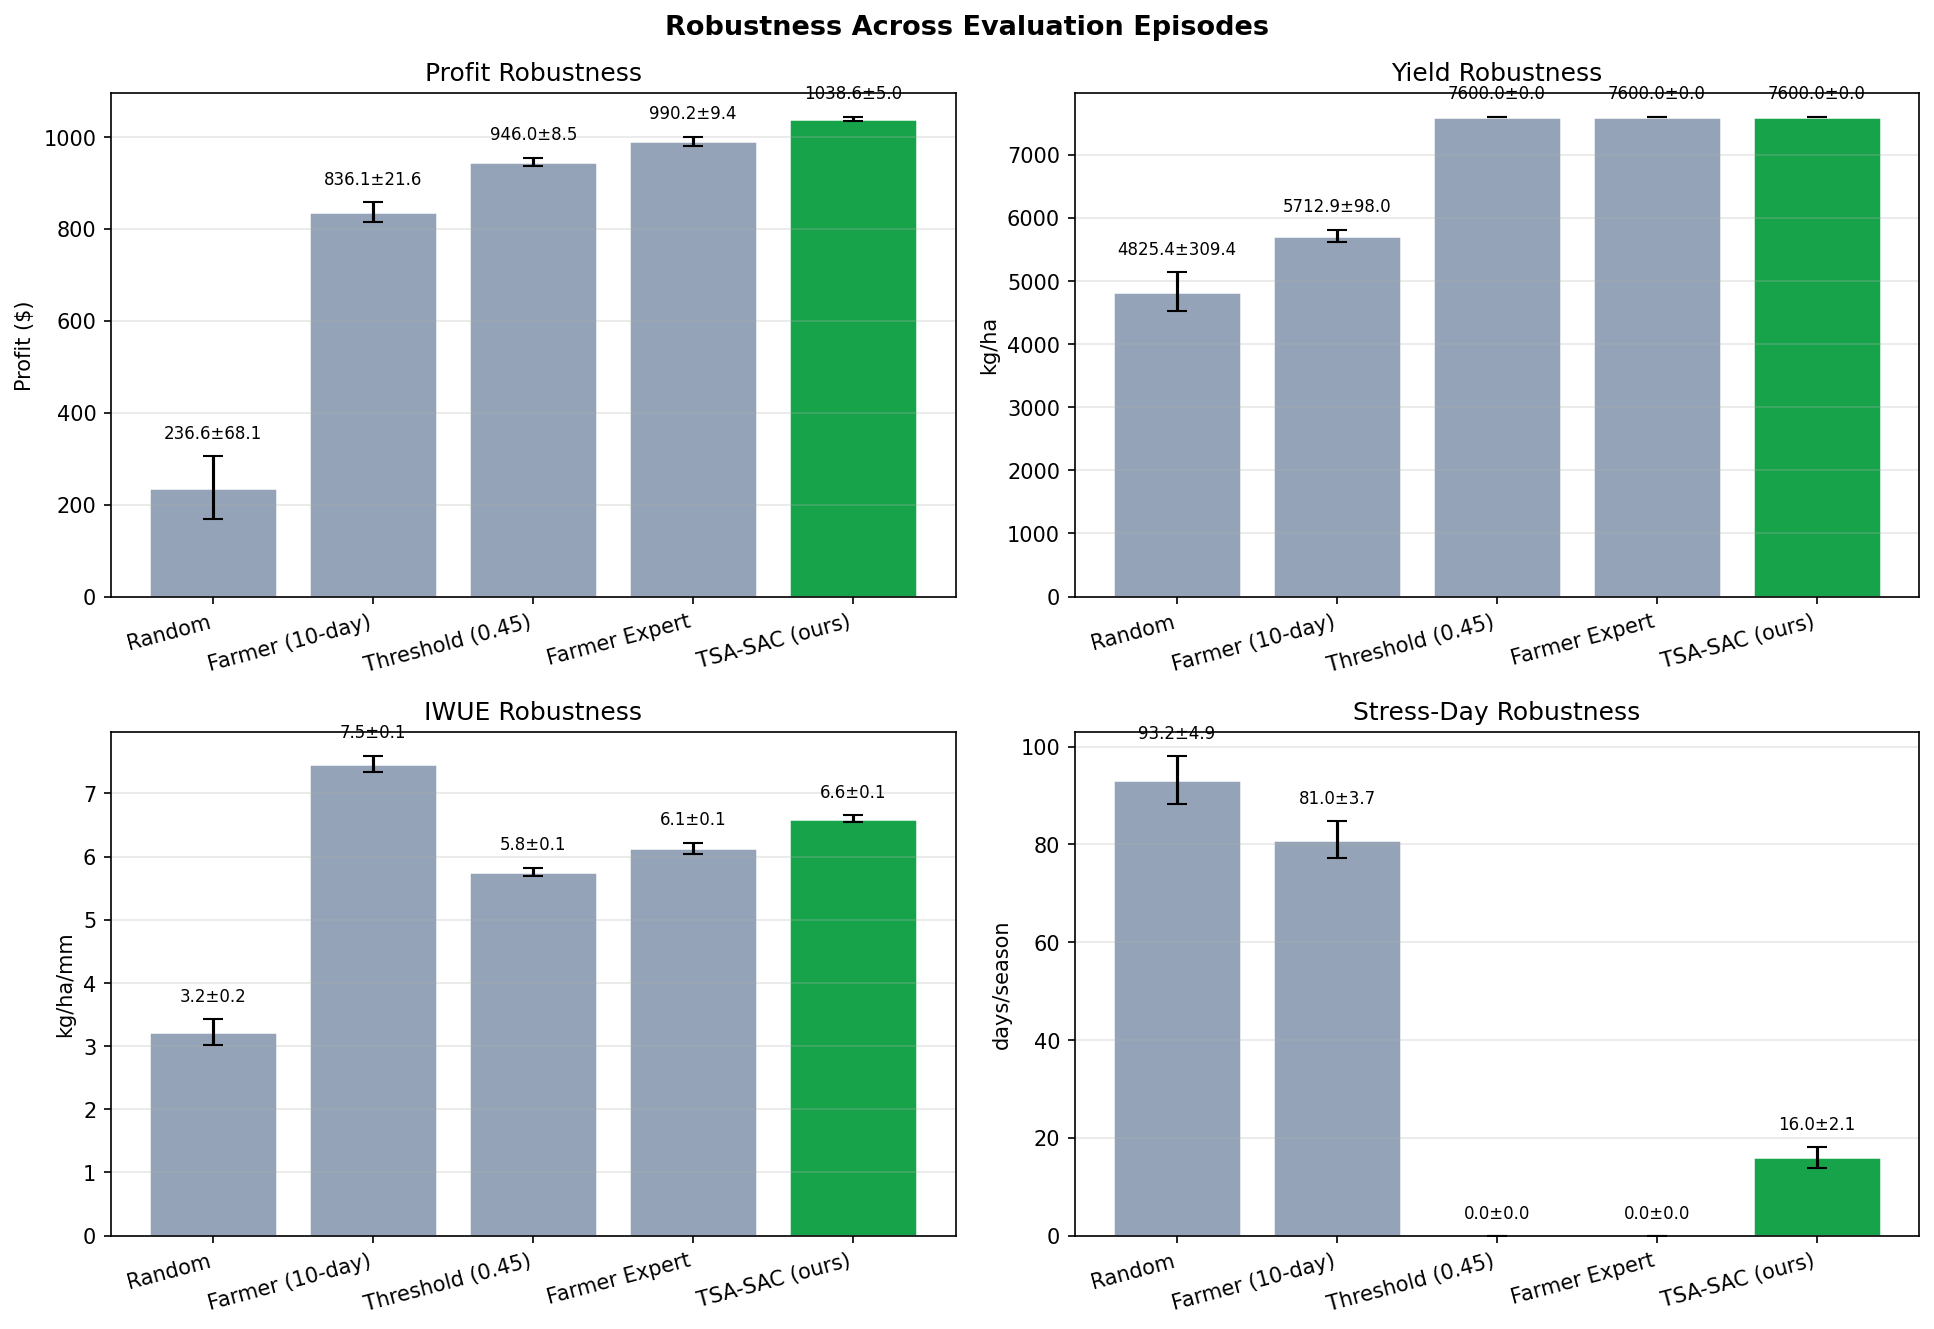
\includegraphics[width=0.85\textwidth]{robustness_analysis.png}
\caption{Robustness Analysis across Weather Variability}
\label{fig:robust}
\end{figure}

Figure~\ref{fig:unseen} breaks down performance across the four scenarios, while Figure~\ref{fig:robust} examines the agent's sensitivity to weather variability within each climate. Together, these results demonstrate that the agent transfers useful irrigation strategies even to conditions it was never exposed to during training.

%================================================================
\section{Conclusion}

We presented TSA-SAC, a temporal-state-aware deep reinforcement learning agent for smart irrigation scheduling. Our agent achieves:
\begin{itemize}
    \item \textbf{\$1,039/ha} season profit---highest among all tested policies
    \item \textbf{1,152\,mm} irrigation---7\% less water than the best expert heuristic
    \item \textbf{6.60 kg/ha/mm} IWUE---8\% better water use efficiency than expert
\end{itemize}

The ablation study confirms that SAC is the right algorithm for continuous irrigation control (SAC $\gg$ PPO by 136\%), and the TSA temporal encoder provides measurable benefit (+1.7\%) by capturing multi-day weather patterns. The hyperparameter analysis reveals that 7-day sequence context contributes a +15\% profit gain over a memoryless agent, validating the BiLSTM design choice. Generalization experiments demonstrate that the policy transfers gracefully to unseen climates and water constraints without retraining.

%================================================================
\section{Future Scope}

\begin{enumerate}
    \item \textbf{Joint Irrigation-Fertilization}: Extend the action space to include nitrogen management for multi-objective optimization
    \item \textbf{Real Crop Model Integration}: Connect to DSSAT or AquaCrop for higher-fidelity simulation and real-world validation
    \item \textbf{Climate Change Scenarios}: Train under projected future weather patterns for robust long-term strategies
    \item \textbf{Multi-Zone Coordination}: Extend to multi-field settings with shared water resources and canal scheduling \cite{zhang2021multizone}
    \item \textbf{Market Price Uncertainty}: Incorporate stochastic crop prices for risk-aware irrigation policies
    \item \textbf{Transfer Learning}: Pre-train on one crop/climate and fine-tune for new conditions with minimal data \cite{gupta2022transfer}
    \item \textbf{Federated Learning}: Train agents across distributed farms while preserving data privacy
    \item \textbf{Real Sensor Integration}: Deploy on IoT-enabled farms with real-time soil moisture and weather data \cite{zhang2021iot}
\end{enumerate}

%================================================================
\begin{thebibliography}{17}

\bibitem{liu2025}
J.~Liu, H.~Zhang, Y.~Wang, and X.~Chen, ``Smart Irrigation Scheduling Using Crop Model and Improved Deep Reinforcement Learning,'' \textit{Agriculture}, vol.~15, no.~24, p.~2569, 2025.

\bibitem{haarnoja2018sac}
T.~Haarnoja, A.~Zhou, P.~Abbeel, and S.~Levine, ``Soft Actor-Critic: Off-Policy Maximum Entropy Deep Reinforcement Learning with a Stochastic Actor,'' in \textit{Proc.\ ICML}, 2018, pp.~1861--1870.

\bibitem{schulman2017ppo}
J.~Schulman, F.~Wolski, P.~Dhariwal, A.~Radford, and O.~Klimov, ``Proximal Policy Optimization Algorithms,'' \textit{arXiv:1707.06347}, 2017.

\bibitem{fujimoto2018td3}
S.~Fujimoto, H.~van Hoof, and D.~Meger, ``Addressing Function Approximation Error in Actor-Critic Methods,'' in \textit{Proc.\ ICML}, 2018, pp.~1587--1596.

\bibitem{fao56}
R.~G.~Allen, L.~S.~Pereira, D.~Raes, and M.~Smith, ``Crop Evapotranspiration---FAO Irrigation and Drainage Paper 56,'' FAO, Rome, 1998.

\bibitem{mnih2015dqn}
V.~Mnih et al., ``Human-Level Control through Deep Reinforcement Learning,'' \textit{Nature}, vol.~518, pp.~529--533, 2015.

\bibitem{chen2021rl}
S.~Chen, L.~He, and X.~Wang, ``Reinforcement Learning-Based Irrigation Scheduling in a Greenhouse Environment,'' \textit{Agricultural Water Management}, vol.~245, p.~106651, 2021.

\bibitem{overweg2021crop}
H.~Overweg, C.~Izzo, S.~Brogaard, J.~E.~Olesen, and M.~Troldborg, ``Crop Model-Based Reinforcement Learning for Intelligent Irrigation,'' in \textit{NeurIPS Workshop on Tackling Climate Change with AI}, 2021.

\bibitem{tao2022multi}
Y.~Tao, X.~Wang, and W.~Liu, ``Multi-Objective Deep Reinforcement Learning for Crop Irrigation Scheduling,'' \textit{Computers and Electronics in Agriculture}, vol.~201, p.~107272, 2022.

\bibitem{xu2020bilstm}
J.~Xu, Z.~Li, and H.~Wang, ``BiLSTM-Attention for Crop Yield Prediction from Sequential Remote Sensing Data,'' \textit{IEEE Geoscience and Remote Sensing Letters}, vol.~18, no.~5, pp.~889--893, 2020.

\bibitem{xu2020energyrl}
X.~Xu, Y.~Jia, Y.~Xu, Z.~Xu, S.~Chai, and C.~S.~Lai, ``A Multi-Agent Reinforcement Learning-Based Data-Driven Method for Home Energy Management,'' \textit{IEEE Transactions on Smart Grid}, vol.~11, no.~4, pp.~3201--3211, 2020.

\bibitem{mahler2020water}
R.~Mahler and J.~Kofman, ``Reinforcement Learning for Irrigation Decisions Under Water Budget Constraints,'' \textit{Environmental Modelling \& Software}, vol.~130, p.~104714, 2020.

\bibitem{nevavuori2020crop}
P.~Nevavuori, N.~Narra, P.~Linna, and T.~Lipping, ``Crop Yield Prediction Using Multitemporal UAV Data and Spatio-Temporal Deep Learning Models,'' \textit{Remote Sensing}, vol.~12, no.~8, p.~1311, 2020.

\bibitem{zhang2021iot}
Y.~Zhang, L.~Wu, and S.~Guo, ``Smart Irrigation System Based on IoT and Deep Learning,'' \textit{IEEE Access}, vol.~9, pp.~54158--54168, 2021.

\bibitem{zhang2021multizone}
Q.~Zhang, Z.~Chen, and F.~Li, ``Multi-Zone Irrigation Coordination Using Deep Reinforcement Learning with Shared Water Resources,'' \textit{Agricultural Systems}, vol.~190, p.~103132, 2021.

\bibitem{vaswani2017}
A.~Vaswani, N.~Shazeer, N.~Parmar, J.~Uszkoreit, L.~Jones, A.~N.~Gomez, L.~Kaiser, and I.~Polosukhin, ``Attention Is All You Need,'' in \textit{Advances in Neural Information Processing Systems}, 2017, pp.~5998--6008.

\bibitem{gupta2022transfer}
A.~Gupta, R.~Kumar, and S.~Singh, ``Transfer Learning for Data-Efficient Crop Management Under Changing Climate Conditions,'' \textit{Computers and Electronics in Agriculture}, vol.~198, p.~107031, 2022.

\end{thebibliography}

\end{document}
